\documentclass[12pt]{article}

% ══════════════════════════════════════════════════════════════
%  FORMATO Y DISEÑO
% ══════════════════════════════════════════════════════════════
\usepackage[top=2.5cm, bottom=3.2cm, outer=3cm, inner=3cm]{geometry}
\usepackage{ragged2e}
\usepackage[spanish]{babel}
\usepackage[defaultfam,tabular,lining]{montserrat}
\usepackage[T1]{fontenc}
\usepackage{xcolor}
\usepackage{tocloft}
\usepackage{setspace}
\usepackage{fancyhdr}
\usepackage{caption}
\usepackage{makeidx}
\makeindex

% ══════════════════════════════════════════════════════════════
%  TABLAS
% ══════════════════════════════════════════════════════════════
\usepackage{array}
\usepackage{tabularx}
\usepackage{multirow}
\usepackage{booktabs}
\usepackage{longtable}
\usepackage{colortbl}
\usepackage{pdflscape}
\usepackage{multicol}

% ══════════════════════════════════════════════════════════════
%  GRÁFICOS Y FIGURAS
% ══════════════════════════════════════════════════════════════
\usepackage{graphicx}
\usepackage{float}
\usepackage{tikz}
\AtBeginDocument{\shorthandoff{>}}
\usetikzlibrary{shapes.geometric, arrows.meta, positioning, decorations.markings}
\usepackage{pgfplots}
\pgfplotsset{compat=1.18}

% ══════════════════════════════════════════════════════════════
%  MATEMÁTICAS
% ══════════════════════════════════════════════════════════════
\usepackage{mathtools}
\usepackage{amsmath}
\usepackage{amsthm}
\usepackage{amssymb}
\usepackage{amsbsy}
\usepackage{amsfonts}
\usepackage{amstext}
\usepackage{amscd}
\usepackage{nccmath}
\usepackage{bbm}
\usepackage{esint}
\usepackage{cancel}
\usepackage{braket}
\usepackage{tensor}
\usepackage{siunitx}
\sisetup{output-decimal-marker={.}, group-separator={,}}
\setcounter{MaxMatrixCols}{30}

% ══════════════════════════════════════════════════════════════
%  QUÍMICA
% ══════════════════════════════════════════════════════════════
\usepackage{chemfig}
\usepackage[version=4]{mhchem}
% chemmacros v6.2a (texlive 2026) rompe el índice al cargar módulo nomenclature
% internamente — reactivar cuando se actualice a v6.3+
% \usepackage{chemmacros}
% \usepackage{chemgreek}
% \chemsetup{modules={redox,thermodynamics,isotopes,iupac}}
\usepackage{elements}
\usepackage{chemnum}
% chemarr rompe el índice en combinación con tocloft — reactivar con chemmacros
% \usepackage{chemarr}
\usepackage{chemplants}
\usepackage{carbohydrates}
\usepackage{chemobabel}
\usepackage{tikzorbital}
\usepackage{modiagram}
% ghsystem rompe el índice vía módulo nomenclature de chemmacros
% Usar PNGs de /usr/share/texmf-dist/tex/latex/ghsystem/pictures/ con \includegraphics
% o cargar manualmente en documentos sin \tableofcontents
% \usepackage{ghsystem}

% -- Estilo ddbond: enlace deslocalizado --
\catcode`\_=11
\tikzset{
ddbond/.style args={#1}{
draw=none,
decoration={%
markings,
mark=at position 0 with {
\coordinate (CF@startdeloc) at (0,\dimexpr#1\CF_doublesep/2)
coordinate (CF@startaxis) at (0,\dimexpr-#1\CF_doublesep/2);
},
mark=at position 1 with {
\coordinate (CF@enddeloc) at (0,\dimexpr#1\CF_doublesep/2)
coordinate (CF@endaxis) at (0,\dimexpr-#1\CF_doublesep/2);
\draw[dash pattern=on 2pt off 1.5pt] (CF@startdeloc)--(CF@enddeloc);
\draw (CF@startaxis)--(CF@endaxis);
}
},
postaction={decorate}
}
}
\catcode`\_=8

% ══════════════════════════════════════════════════════════════
%  DIAMANTE NFPA 704
% ══════════════════════════════════════════════════════════════
% Uso: \NFPAdiamond{salud}{inflamab}{reactividad}{especial}
\newcommand{\NFPAdiamond}[4]{%
    \begin{tikzpicture}[scale=0.45, every node/.style={transform shape}]
        \draw[thick, line width=1.5pt] (0,2) -- (2,4) -- (4,2) -- (2,0) -- cycle;
        \draw[thick] (0,2) -- (4,2);
        \draw[thick] (2,0) -- (2,4);
        \fill[red]    (2,4) -- (1,3) -- (2,2) -- (3,3) -- cycle;
        \node[text=white, font=\bfseries\Large] at (2,3.1)  {#2};
        \fill[blue]   (0,2) -- (1,3) -- (2,2) -- (1,1) -- cycle;
        \node[text=white, font=\bfseries\Large] at (0.9,2)  {#1};
        \fill[yellow] (4,2) -- (3,3) -- (2,2) -- (3,1) -- cycle;
        \node[text=black, font=\bfseries\Large] at (3.1,2)  {#3};
        \fill[white]  (2,0) -- (1,1) -- (2,2) -- (3,1) -- cycle;
        \node[text=black, font=\bfseries\large] at (2,0.9)  {#4};
        \draw[thick, line width=1.5pt] (0,2) -- (2,4) -- (4,2) -- (2,0) -- cycle;
    \end{tikzpicture}%
}

% ══════════════════════════════════════════════════════════════
%  CAJAS Y RESALTADO
% ══════════════════════════════════════════════════════════════
\usepackage[most]{tcolorbox}

% ══════════════════════════════════════════════════════════════
%  REFERENCIAS Y ENLACES
% ══════════════════════════════════════════════════════════════
\usepackage[utf8]{inputenc}
\usepackage{csquotes}
\usepackage[hidelinks]{hyperref}
\usepackage{url}
\usepackage{enumitem}
\usepackage{fancyvrb}
\usepackage{cleveref}
\usepackage{witharrows}
\usepackage{microtype}
\usepackage[backend=biber, style=apa, language=spanish]{biblatex}

\allowdisplaybreaks

% ══════════════════════════════════════════════════════════════
%  COLORES
% ══════════════════════════════════════════════════════════════
\definecolor{blueunam}{RGB}{50, 70, 90}
\definecolor{catred}{RGB}{192,57,43}
\definecolor{anblue}{RGB}{41,128,185}
\definecolor{col1}{RGB}{210,228,255}
\definecolor{col2}{RGB}{200,238,210}
\definecolor{trans}{RGB}{255,238,200}
\definecolor{trans2}{RGB}{255,220,185}
\definecolor{pos}{RGB}{228,218,255}
\definecolor{especial}{RGB}{235,235,235}

% ══════════════════════════════════════════════════════════════
%  ENCABEZADO Y PIE DE PÁGINA
% ══════════════════════════════════════════════════════════════
\pagestyle{fancy}
\fancyhf{}
\fancyfoot[R]{\thepage}
% -- Encabezado con materia y sección activa (descomentar para activar) --
% \fancyhead[L]{\small\textcolor{blueunam}{Nombre de la materia}}
% \fancyhead[R]{\small\textcolor{blueunam}{\leftmark}}
% \renewcommand{\headrulewidth}{0.4pt}
% \renewcommand{\headrule}{\hbox to\headwidth{\color{blueunam}\leaders\hrule height \headrulewidth\hfill}}
\renewcommand{\headrulewidth}{0pt}

\renewcommand*\oldstylenums[1]{{\fontfamily{Montserrat-TOsF}\selectfont #1}}

% ══════════════════════════════════════════════════════════════
%  ÍNDICE Y BIBLIOGRAFÍA
% ══════════════════════════════════════════════════════════════
\AtBeginDocument{
    \renewcommand{\contentsname}{
        \centering\fontsize{12}{18}\selectfont
        \textcolor{blueunam}{\textbf{ÍNDICE}}
    }
}
\AtBeginDocument{
    \renewcommand{\bibname}{
        \centering\fontsize{12}{18}\selectfont
        \textcolor{blueunam}{\textbf{REFERENCIAS}}
    }
}
\renewcommand{\cftsecfont}{\color{blueunam}}
\setcounter{tocdepth}{3}
\setcounter{secnumdepth}{3}

% ══════════════════════════════════════════════════════════════
%  COLUMNAS PERSONALIZADAS
% ══════════════════════════════════════════════════════════════
\newcolumntype{L}[1]{>{\raggedright\arraybackslash}p{#1}}
\newcolumntype{C}[1]{>{\centering\arraybackslash}p{#1}}

% ══════════════════════════════════════════════════════════════
%  CELDAS DE TABLA DE CATIONES
% ══════════════════════════════════════════════════════════════
% Uso: \catcell{color}{símbolo}{Z}{carga/nombre}
\newcommand{\catcell}[4]{%
    \cellcolor{#1}%
    \begin{minipage}[t][1.8cm][t]{1.6cm}%
        \centering\vspace{3pt}%
        {\small\textbf{#2}}\\[2pt]%
        {\tiny\color{gray}#3}\\[3pt]%
        {\footnotesize\color{blueunam}#4}%
    \end{minipage}}

\newcommand{\emptycell}{%
    \cellcolor{white}%
    \begin{minipage}[t][1.8cm][t]{1.6cm}\end{minipage}}

% ══════════════════════════════════════════════════════════════
%  AMBIENTE DE EJERCICIOS
% ══════════════════════════════════════════════════════════════
\newtcbtheorem{exercise}{Ejercicio}{
    enhanced,frame empty,interior empty,
    colframe=blueunam,
    borderline west={1pt}{0pt}{blueunam},
    left=0.2cm,
    attach boxed title to top left={yshift=-2mm,xshift=-2mm},
    coltitle=black,
    fonttitle=\bfseries,
    colbacktitle=white,
    boxed title style={boxrule=.4pt,sharp corners}}{exercise}

% ══════════════════════════════════════════════════════════════
%  PIES DE FIGURA Y TABLA (APA)
% ══════════════════════════════════════════════════════════════
\DeclareCaptionLabelSeparator*{spaced}{\\[2ex]}
\captionsetup[table]{textfont=it,format=plain,justification=justified,
  singlelinecheck=false,labelsep=spaced,skip=0pt}
\captionsetup[figure]{labelsep=period,labelfont=bf,justification=justified,
  singlelinecheck=false,font=doublespacing}

\setlength{\parindent}{0pt}

% ══════════════════════════════════════════════════════════════
%  DOCUMENTO
% ══════════════════════════════════════════════════════════════
\begin{document}

%---------- Portada ----------%
\begin{titlepage}
\thispagestyle{empty}
\begin{center}
\vspace*{2cm}
\fontsize{14}{30}\selectfont\textbf{Universidad Nacional Autónoma de México} \\
\vspace{1cm}
\fontsize{14}{30}\selectfont\textbf{Química e Ingeniería en Materiales} \\
\vspace{1cm}
\fontsize{14}{30}\selectfont\textbf{Química de Materiales} \\
\end{center}
\vspace{2cm}
\begin{flushright}
    \fontsize{14}{30}\selectfont
        \hspace{2cm} Nombre: Uriel Sánchez Méndez \\
        \hspace{2cm} Matrícula: 322647576 \\
        \hspace{2cm} Apuntes de Química de Materiales \\
        \hspace{2cm} Fecha: \today \\
\end{flushright}
\end{titlepage}

%---------- Tabla de contenido ----------%
\tableofcontents
\thispagestyle{empty}
\newpage

%---------- Apuntes ----------%
\spacing{1.5}
\phantomsection
\addcontentsline{toc}{subsection}{Fundamentos Previos}
\fontsize{12}{18}\selectfont{\textcolor{blueunam}{\textbf{QUÍMICA DE MATERIALES}}}
\subsection*{\textcolor{blueunam}{Fundamentos Previos}}

\phantomsection
\addcontentsline{toc}{subsubsection}{Tipos de enlace}
\subsubsection*{\textcolor{blueunam}{Tipos de enlace}}

\textbf{Enlace covalente:} interacción entre dos átomos en la que sus 
orbitales atómicos se solapan en fase, sumando constructivamente las 
funciones de onda y aumentando la densidad electrónica entre los núcleos. 
Esa densidad es atraída por ambos núcleos positivos, bajando la energía 
potencial del sistema. Si esa estabilización supera la repulsión 
núcleo-núcleo, el sistema se estabiliza y existe el enlace. Los átomos 
comparten uno o más pares de electrones, generalmente uno por átomo. 
Se considera covalente cuando la diferencia de electronegatividad es 
menor a 1.7.

\begin{center}
\schemestart
\chemname{\chemfig{H-C(-[2]H)(-[6]H)-H}}{Metano \ce{CH4}}
\schemestop
\end{center}

\textbf{Enlace sencillo:} enlace covalente en el que dos átomos comparten 
exactamente un par de electrones mediante solapamiento frontal de orbitales, 
formando un enlace $\sigma$. Es el enlace de menor orden (O.E.$=1$) y 
permite rotación libre alrededor del eje internuclear.

\begin{center}
\schemestart
\chemname{\chemfig{H-H}}{\ce{H2}, enlace $\sigma$}
\schemestop
\end{center}

\textbf{Enlace polar:} enlace covalente en el que los electrones no se 
distribuyen simétricamente porque los átomos tienen distinta 
electronegatividad. El más electronegativo concentra mayor densidad 
electrónica ($\delta^-$) y el otro queda con una deficiencia ($\delta^+$), 
generando un dipolo de enlace. Si los dipolos se cancelan vectorialmente 
por la geometría molecular, la molécula tiene momento dipolar neto igual 
a cero.

\begin{center}
\schemestart
\chemname{\chemfig{H-[104.5]\charge{45=\:,135=\:}{O}-[-104.5]H}}{Ejemplo: \ce{H2O}, geometría angular, dipolos no se cancelan, $\mu \neq 0$}
\schemestop
\end{center}

\begin{center}
\schemestart
\chemname{\chemfig{O=C=O}}{Contraejemplo: \ce{CO2}, geometría lineal, dipolos se cancelan, $\mu = 0$}
\schemestop
\end{center}

\textbf{Estructura de Lewis:} representación que muestra explícitamente 
todos los electrones de valencia de una molécula o ion. Los compartidos 
se representan como líneas entre átomos, cada una valiendo 2 electrones, 
y los no compartidos como pares libres sobre cada átomo. Se construye 
distribuyendo los electrones de valencia totales minimizando cargas formales.

\begin{center}
\schemestart
\chemname{\chemfig{H-\charge{90=\:}{N}(-[6]H)-H}}{\ce{NH3}: $e^-_T = 5+(1\times3) = 8$, C.F. N $= 5-2-3 = 0$, C.F. H $= 0$}
\schemestop
\end{center}


\phantomsection
\addcontentsline{toc}{subsubsection}{Carga formal vs densidad electrónica real}
\subsubsection*{\textcolor{blueunam}{Carga formal vs densidad electrónica real}}

La \textbf{carga formal} es un conteo entero: cuántos electrones completos 
le sobran o faltan a un átomo respecto a su estado neutro, asumiendo que 
los electrones enlazantes se dividen exactamente a la mitad. Es una 
convención útil para verificar estructuras de Lewis, no una medida de 
distribución real.

En realidad los electrones no ``pertenecen'' fijamente a ningún átomo: 
son probabilísticos. Lo que sí es real es que estadísticamente, en promedio, 
ciertos átomos concentran más densidad electrónica que otros. Eso se 
describe con la carga parcial $\delta$: un átomo con más densidad promedio 
tiene $\delta^-$, uno con menos tiene $\delta^+$. Si la diferencia es mayor, 
la carga parcial es mayor, pero siempre es un promedio estadístico, nunca 
un valor discreto fijo como en la carga iónica real.

\textbf{En enlaces iónicos} como \ce{NaCl}, la carga sí es real: el 
\ce{Na+} físicamente perdió un electrón y tiene 10 electrones. En 
covalente, la carga formal \ce{+1} o \ce{-1} no implica transferencia 
real, solo un déficit en el conteo convencional.

\begin{center}
\small
\renewcommand{\arraystretch}{1.4}
\begin{tabular}{|L{3.5cm}|L{4cm}|L{4cm}|}
\hline
\textbf{Concepto} & \textbf{Qué describe} & \textbf{Ejemplo} \\
\hline
Carga formal & Conteo entero de electrones de más o de menos & 
\ce{O} en \ce{OH-}: C.F. $= -1$ \\
\hline
Carga parcial $\delta$ & Probabilidad de encontrar densidad en un átomo & 
\ce{C-O}: $\delta^+$ en C, $\delta^-$ en O \\
\hline
Carga iónica real & Transferencia física de un electrón completo & 
\ce{Na+} en \ce{NaCl}: realmente tiene 10 $e^-$ \\
\hline
\end{tabular}
\normalsize
\end{center}

%---------- Apuntes ----------%
\spacing{1.5}
\phantomsection
\addcontentsline{toc}{section}{Apuntes}
\begin{center}
\end{center}

\phantomsection
\addcontentsline{toc}{subsection}{Unidad 1. Fundamentos de Química}
\subsection*{\textcolor{blueunam}{Unidad 1. Fundamentos de Química}}

\phantomsection
\addcontentsline{toc}{subsubsection}{Clase 1 -- 18/08/2026: Definiciones y conceptos básicos}
\subsubsection*{\textcolor{blueunam}{Clase 1 -- 18/08/2026: Definiciones y conceptos básicos}}

Reactivo: Sustancia que puede interactuar o reaccionar con otra sustancia. (Se transforma --> Proceso de una sustancia para formar otra.) Un producto también puede actuar como reactivo A + B $\longleftrightarrow$  C $\rightarrow$ D \\
Sustrato o Materia prima: es la especie o reactivo específico sobre el cual actúa otro compuesto (un reactivo o catalizador) para transformarse en un producto, mientras que la materia prima química es el insumo base general. \\

Ejemplo:
\begin{center}
\schemestart
\chemfig{*6(-=-=-=)}
\arrow{->[\ce{HNO3}][\ce{H2SO4}]}
\chemfig{*6(-=(-NO_2)-=-=)}
\schemestop
\end{center}

El sustrato o Materia prima es la que se conserva en este caso la molécula de benceno es la que se conserva \\
Reactivo: Benceno, ácido nítrico y ácido sulfúrico \\
Producto: Nitrobenceno \\

Todo sustrato es un Reactivo, pero no todo Reactivo es un Sustrato. \\

\begin{center}
\schemestart
\chemname{\chemfig{*6(-=*5(-N(-H)-==-)-=-=-)}}{Indol}
\arrow{->[\shortstack{\ce{NBS}\\\small reactivo}][\shortstack{\ce{DMF}\\\small medio}]}
\chemname{\chemfig{*6(-=*5(-N(-H)-==-)-=(-Br)-=-)}}{5-bromoindol}
\+
\chemname{\chemfig{*6(-=*5(-N(-H)-=(-Br)=-)-=(-Br)-=-)}}{3,5-dibromoindol}
\schemestop
\end{center}

Producto: Sustancia final de la reacción ``(Es de interés)'' \\
Subproducto: Sustancia residual o no deseada de la reacción \\

\phantomsection
\addcontentsline{toc}{subsubsection}{Clase 2 -- 20/08/2026: Especies reactivas}
\subsubsection*{\textcolor{blueunam}{Clase 2 -- 20/08/2026: Especies reactivas}}

A $\rightarrow$ B (70\,\%) + C (20\,\%) + D (10\,\%) \\
Producto de interés $\neq$ Producto principal \\ 

Especies Reactivas: Especies que aparecen durante la reacción, pero desaparece al final. \\

\begin{itemize}
    \item \textcolor{blueunam}{\textbf{1- Carbocationes}}
    \item \textcolor{blueunam}{\textbf{2- Carbaniones}}
    \item \textcolor{blueunam}{\textbf{3- Radicales}}
    \item \textcolor{blueunam}{\textbf{4- Carbenos}}
\end{itemize}

\textcolor{blueunam}{\textbf{1- Carbocationes}}

\begin{center}
\schemestart
\chemfig{R-C^{\color{catred}+}(-[2]R)(-[6]R)}
\schemestop
\end{center}

\ce{e^{\color{anblue}-}} $-$ \ce{e^{\color{anblue}-}} libres $-$ \#enlaces $=$ Carga del átomo

Geometría (E.V.) \\

Repaso E.V.: 
Flujo de trabajo: \\
\begin{itemize}
    \item 1-Lewis
    \item 2-TRPECV
    \item 3-T.E.V.
    \item 4-T.O.M.
\end{itemize}

Lewis: \\
\begin{center}
\begin{tabular}{ll}
$\text{H}_2\text{O}$ & \\[6pt]
$\begin{array}{r}
2\,\ce{e^{\color{anblue}-}} \\
+\,6\,\ce{e^{\color{anblue}-}} \\
\hline
8\,\ce{e^{\color{anblue}-}} \\
-\,4\,\ce{e^{\color{anblue}-}} \\
\hline
4\,\ce{e^{\color{anblue}-}} \\
-\,4\,\ce{e^{\color{anblue}-}} \\
\hline
0\,\ce{e^{\color{anblue}-}}
\end{array}$
&
\chemfig{H-\charge{45=\:,135=\:}{O}-H}
\end{tabular}
\end{center}

\[
\begin{array}{rl}
\text{C.F. O} & = 6 - 2 - 4 = 0 \\
\text{C.F. H} & = (1 - 1 - 0) \times 2 = 0 \\
\hline
\text{Carga total} & = 0
\end{array}
\]

TRPECV: \\
Debido a que tiene 4 especies y 2 de ellas son pares de electrones
libres entonces la geometría es angular y podríamos sacar la hibridación
esperada que sería la $sp^3$ \\
\begin{center}
\chemfig{H-[104.5]\charge{45=\:,135=\:}{O}-[-104.5]H}
\end{center}

T.E.V.: \\
\ce{O}:$1s^2 2s^2 2p^4$ 


\begin{center}
\begin{tikzpicture}
\shorthandoff{>}

% --- Configuración original ---
% 1s
\draw (0,0) rectangle (0.8,0.8);
\node at (0.4,0.4) {$\upharpoonleft\downharpoonright$};
\node at (0.4,-0.3) {\small 1s};

% 2s
\draw (1.2,0) rectangle (2,0.8);
\node at (1.6,0.4) {$\upharpoonleft\downharpoonright$};
\node at (1.6,-0.3) {\small 2s};

% 2px
\draw (2.4,0) rectangle (3.2,0.8);
\node at (2.8,0.4) {$\upharpoonleft\downharpoonright$};
\node at (2.8,-0.3) {\small $2p_x$};

% 2py
\draw (3.4,0) rectangle (4.2,0.8);
\node at (3.8,0.4) {$\upharpoonleft$};
\node at (3.8,-0.3) {\small $2p_y$};

% 2pz
\draw (4.6,0) rectangle (5.4,0.8);
\node at (5,0.4) {$\upharpoonleft$};
\node at (5,-0.3) {\small $2p_z$};

% Flecha hibridación
\draw[-{Stealth}, thick] (5.8,0.4) -- (8.6,0.4);
\node at (7.2,0.7) {Hibridación};

% --- Configuración hibridada ---
% 1s (no cambia)
\draw (9.0,0) rectangle (9.8,0.8);
\node at (9.4,0.4) {$\upharpoonleft\downharpoonright$};
\node at (9.4,-0.3) {\small 1s};

% sp2 - caja 1
\draw (10.2,0) rectangle (11.0,0.8);
\node at (10.6,0.4) {$\upharpoonleft\downharpoonright$};
\node at (10.6,-0.3) {\small $sp^3$};

% sp2 - caja 2
\draw (11.4,0) rectangle (12.2,0.8);
\node at (11.8,0.4) {$\upharpoonleft\downharpoonright$};
\node at (11.8,-0.3) {\small $sp^3$};

% sp2 - caja 3
\draw (12.6,0) rectangle (13.4,0.8);
\node at (13.0,0.4) {$\upharpoonleft$};
\node at (13.0,-0.3) {\small $sp^3$};

% 2pz
\draw (13.8,0) rectangle (14.6,0.8);
\node at (14.2,0.4) {$\upharpoonleft$};
\node at (14.2,-0.3) {\small $sp^3$};

\end{tikzpicture}
\end{center}

Sé que es sp³ porque el átomo central tiene 4 grupos (2 pares libres + 2 enlaces). 
El número de grupos debe coincidir con el número de orbitales híbridos. 
El 1s no participa porque es un orbital de core (baja energía, no de valencia). 
Se hibridan 2s + 2px + 2py + 2pz: 1 orbital s y 3 orbitales p → sp³. \\

\textbf{La hibridación del carbono en el carbocatión:} \\

\begin{center}
\schemestart
\chemname{\chemfig{R-C^{\color{catred}+}(-[2]R)(-[6]R)}}{Carbocatión}
\schemestop
\end{center}

E.V. del carbocatión: \\
\ce{C}: $1s^2\,2s^2\,2p^2$ \textit{\textbf{(importante recordar que el carbono está cargado positivamente, así que la configuración cambia)}} $\rightarrow$ C$^{\color{catred}+}$: $1s^2\,2s^2\,2p^1$

\begin{center}
\begin{tikzpicture}
\shorthandoff{>}

% --- Fila 1: Original → Promoción ---
% 1s
\draw (0,0) rectangle (0.8,0.8);
\node at (0.4,0.4) {$\upharpoonleft\downharpoonright$};
\node at (0.4,-0.3) {\small 1s};

% 2s
\draw (1.2,0) rectangle (2,0.8);
\node at (1.6,0.4) {$\upharpoonleft\downharpoonright$};
\node at (1.6,-0.3) {\small 2s};

% 2px
\draw (2.4,0) rectangle (3.2,0.8);
\node at (2.8,0.4) {$\upharpoonleft$};
\node at (2.8,-0.3) {\small $2p_x$};

% 2py vacío
\draw (3.4,0) rectangle (4.2,0.8);
\node at (3.8,-0.3) {\small $2p_y$};

% 2pz vacío
\draw (4.6,0) rectangle (5.4,0.8);
\node at (5,-0.3) {\small $2p_z$};

% Flecha promoción
\draw[-{Stealth}, thick] (5.8,0.4) -- (8.6,0.4);
\node at (7.2,0.7) {Promoción};

% --- Configuración promovida ---
% 1s
\draw (9.0,0) rectangle (9.8,0.8);
\node at (9.4,0.4) {$\upharpoonleft\downharpoonright$};
\node at (9.4,-0.3) {\small 1s};

% 2s con 1 electrón
\draw (10.2,0) rectangle (11.0,0.8);
\node at (10.6,0.4) {$\upharpoonleft$};
\node at (10.6,-0.3) {\small 2s};

% 2px
\draw (11.4,0) rectangle (12.2,0.8);
\node at (11.8,0.4) {$\upharpoonleft$};
\node at (11.8,-0.3) {\small $2p_x$};

% 2py
\draw (12.6,0) rectangle (13.4,0.8);
\node at (13.0,0.4) {$\upharpoonleft$};
\node at (13.0,-0.3) {\small $2p_y$};

% 2pz vacío
\draw (13.8,0) rectangle (14.6,0.8);
\node at (14.2,-0.3) {\small $2p_z$};

% --- Fila 2: Promoción → Hibridación ---
% 1s
\draw (0,-2.5) rectangle (0.8,-1.7);
\node at (0.4,-2.1) {$\upharpoonleft\downharpoonright$};
\node at (0.4,-2.8) {\small 1s};

% 2s
\draw (1.2,-2.5) rectangle (2,-1.7);
\node at (1.6,-2.1) {$\upharpoonleft$};
\node at (1.6,-2.8) {\small 2s};

% 2px
\draw (2.4,-2.5) rectangle (3.2,-1.7);
\node at (2.8,-2.1) {$\upharpoonleft$};
\node at (2.8,-2.8) {\small $2p_x$};

% 2py
\draw (3.4,-2.5) rectangle (4.2,-1.7);
\node at (3.8,-2.1) {$\upharpoonleft$};
\node at (3.8,-2.8) {\small $2p_y$};

% 2pz vacío
\draw (4.6,-2.5) rectangle (5.4,-1.7);
\node at (5,-2.8) {\small $2p_z$};

% Flecha hibridación
\draw[-{Stealth}, thick] (5.8,-2.1) -- (8.6,-2.1);
\node at (7.2,-1.8) {Hibridación};

% --- Configuración hibridada sp2 ---
% 1s (no cambia)
\draw (9.0,-2.5) rectangle (9.8,-1.7);
\node at (9.4,-2.1) {$\upharpoonleft\downharpoonright$};
\node at (9.4,-2.8) {\small 1s};

% sp2 - caja 1
\draw (10.2,-2.5) rectangle (11.0,-1.7);
\node at (10.6,-2.1) {$\upharpoonleft$};
\node at (10.6,-2.8) {\small $sp^2$};

% sp2 - caja 2
\draw (11.4,-2.5) rectangle (12.2,-1.7);
\node at (11.8,-2.1) {$\upharpoonleft$};
\node at (11.8,-2.8) {\small $sp^2$};

% sp2 - caja 3
\draw (12.6,-2.5) rectangle (13.4,-1.7);
\node at (13.0,-2.1) {$\upharpoonleft$};
\node at (13.0,-2.8) {\small $sp^2$};

% 2pz vacío
\draw (13.8,-2.5) rectangle (14.6,-1.7);
\node at (14.2,-2.8) {\small $2p_z$};

\end{tikzpicture}
\end{center}

Geometría trigonal plana, 120° por ángulo \\


Electrófilo — especie que busca electrones (electron-lover).
Puede ser catión, molécula con carga parcial positiva o átomo
con orbital vacío. No necesariamente tiene carga formal positiva,
solo tiene deficiencia electrónica. \\

Nucleófilo — especie que dona electrones (nucleus-lover).
Tiene par de electrones disponible para compartir. Puede
ser anión, molécula con pares libres o enlace $\pi$. \\

\begin{center}
\begin{tikzpicture}
    % Tres enlaces a 120°
    \draw (0,0) -- (1.5,0) node[right] {R};
    \draw (0,0) -- (-0.75,1.3) node[above left] {R};
    \draw (0,0) -- (-0.75,-1.3) node[below left] {R};

    % Lóbulo superior
    \draw[dashed] (0,0.15) .. controls (-0.35,0.7) and (-0.35,1.3) .. (0,1.4)
                  .. controls (0.35,1.3) and (0.35,0.7) .. (0,0.15);

    % Lóbulo inferior
    \draw[dashed] (0,-0.15) .. controls (-0.35,-0.7) and (-0.35,-1.3) .. (0,-1.4)
                  .. controls (0.35,-1.3) and (0.35,-0.7) .. (0,-0.15);

    % Átomo central encima de todo
    \node[fill=white] at (0,0) {C$^{\color{catred}+}$};

    % Etiqueta
    \node[right] at (0.2,1.0) {\small $2p_z$ vacío};

\end{tikzpicture}

\small Carbocatión --- trigonal plana, $sp^2$, $2p_z$ vacío perpendicular al plano
\end{center}

\textbf{Efecto inductivo:} redistribución de densidad
electrónica a través de enlaces $\sigma$ por diferencia de
electronegatividad entre átomos. El átomo más electronegativo
polariza el enlace hacia sí, transmitiendo el efecto a lo largo
de la cadena con intensidad decreciente. Puede ser estabilizador
(grupos electrodonadores) o desestabilizador (grupos electroatractores)
según la dirección del jalón electrónico. \\

\textbf{Hiperconjugación:} deslocalización parcial de electrones
de un enlace $\sigma$ (C--H o C--C) hacia un orbital $p$ vacío
adyacente mediante solapamiento lateral. Requiere alineación paralela
entre el enlace $\sigma$ y el orbital $p$. Estabiliza al sistema al
aumentar la deslocalización electrónica, reduciendo la energía total.
No es un enlace $\pi$ completo sino una interacción $\sigma \rightarrow p$
de tres centros y dos electrones. \\

\begin{center}
\begin{tikzpicture}[scale=1.4]
\shorthandoff{>}

% --- Carbocatión C+ ---
\draw (0,0) -- (-0.75,1.3) node[above left] {H};
\draw (0,0) -- (-0.75,-1.3) node[below left] {H};

% Lóbulo superior pz
\draw[dashed] (0,0.15) .. controls (-0.35,0.7) and (-0.35,1.3) .. (0,1.4)
                  .. controls (0.35,1.3) and (0.35,0.7) .. (0,0.15);

% Lóbulo inferior pz
\draw[dashed] (0,-0.15) .. controls (-0.35,-0.7) and (-0.35,-1.3) .. (0,-1.4)
                  .. controls (0.35,-1.3) and (0.35,-0.7) .. (0,-0.15);

% Enlace C+--CH3
\draw (0,0) -- (2.0,0);
\node[fill=white] at (0,0) {C$^{\color{catred}+}$};

% --- CH3 adyacente ---
\draw (2.0,0) -- (2.0,1.3) node[above] {H};
\draw (2.0,0) -- (2.0,-1.3) node[below] {H};
\draw (2.0,0) -- (3.3,0) node[right] {H};
\node[fill=white] at (2.0,0) {C};

% Etiqueta pz
\node[right] at (0.2,1.0) {\small $2p_z$ vacío};

% Flecha 1: C-H superior → lóbulo superior pz
\draw[-{Stealth}, thick] (2.0,1.1) .. controls (1.2,1.8) and (0.4,1.6) .. (0.1,1.0);

% Flecha 2: C-H inferior → lóbulo inferior pz
\draw[-{Stealth}, thick] (2.0,-1.1) .. controls (1.2,-1.8) and (0.4,-1.6) .. (0.1,-1.0);

\node at (1.0,2.0) {\small Hiperconjugación};

% Puntos enlace C+-C (centrados en el enlace)
\filldraw (0.9,0) circle (1.2pt);
\filldraw (1.1,0) circle (1.2pt);

% Puntos enlace C-H superior (centrados en el enlace)
\filldraw (2.0,0.6) circle (1.2pt);
\filldraw (2.0,0.8) circle (1.2pt);

% Puntos enlace C-H inferior
\filldraw (2.0,-0.6) circle (1.2pt);
\filldraw (2.0,-0.8) circle (1.2pt);

% Puntos enlace C-H lateral
\filldraw (2.6,0) circle (1.2pt);
\filldraw (2.8,0) circle (1.2pt);

\end{tikzpicture}
\end{center}

Tipos de Carbocatión: \\

\begin{center}
\textbf{Carbocatión Primario} \\[6pt]
\begin{tikzpicture}
    % Tres enlaces a 120°
    \draw (0,0) -- (1.5,0) node[right] {H};
    \draw (0,0) -- (-0.75,1.3) node[above left] {$CH_3$};
    \draw (0,0) -- (-0.75,-1.3) node[below left] {H};

    % Lóbulo superior
    \draw[dashed] (0,0.15) .. controls (-0.35,0.7) and (-0.35,1.3) .. (0,1.4)
                  .. controls (0.35,1.3) and (0.35,0.7) .. (0,0.15);

    % Lóbulo inferior
    \draw[dashed] (0,-0.15) .. controls (-0.35,-0.7) and (-0.35,-1.3) .. (0,-1.4)
                  .. controls (0.35,-1.3) and (0.35,-0.7) .. (0,-0.15);

    % Átomo central encima de todo
    \node[fill=white] at (0,0) {C$^{\color{catred}+}$};

    % Etiqueta
    \node[right] at (0.2,1.0) {\small $2p_z$ vacío};

\end{tikzpicture}

\small Carbocatión de tipo primario, tiene 3 interacciones
de hiperconjugación posibles, una por cada enlace C-H del $CH_3$,
que contribuyen por rotación libre del grupo metilo.
\end{center}

\begin{center}
\textbf{Carbocatión Secundario} \\[6pt]
\begin{tikzpicture}
    % Tres enlaces a 120°
    \draw (0,0) -- (1.5,0) node[right] {$CH_3$};
    \draw (0,0) -- (-0.75,1.3) node[above left] {$CH_3$};
    \draw (0,0) -- (-0.75,-1.3) node[below left] {H};

    % Lóbulo superior
    \draw[dashed] (0,0.15) .. controls (-0.35,0.7) and (-0.35,1.3) .. (0,1.4)
                  .. controls (0.35,1.3) and (0.35,0.7) .. (0,0.15);

    % Lóbulo inferior
    \draw[dashed] (0,-0.15) .. controls (-0.35,-0.7) and (-0.35,-1.3) .. (0,-1.4)
                  .. controls (0.35,-1.3) and (0.35,-0.7) .. (0,-0.15);

    % Átomo central encima de todo
    \node[fill=white] at (0,0) {C$^{\color{catred}+}$};

    % Etiqueta
    \node[right] at (0.2,1.0) {\small $2p_z$ vacío};

\end{tikzpicture}

\small Tiene 6 interacciones de hiperconjugación posibles.
\end{center}

\begin{center}
\textbf{Carbocatión Terciario} \\[6pt]
\begin{tikzpicture}
    % Tres enlaces a 120°
    \draw (0,0) -- (1.5,0) node[right] {$CH_3$};
    \draw (0,0) -- (-0.75,1.3) node[above left] {$CH_3$};
    \draw (0,0) -- (-0.75,-1.3) node[below left] {$CH_3$};

    % Lóbulo superior
    \draw[dashed] (0,0.15) .. controls (-0.35,0.7) and (-0.35,1.3) .. (0,1.4)
                  .. controls (0.35,1.3) and (0.35,0.7) .. (0,0.15);

    % Lóbulo inferior
    \draw[dashed] (0,-0.15) .. controls (-0.35,-0.7) and (-0.35,-1.3) .. (0,-1.4)
                  .. controls (0.35,-1.3) and (0.35,-0.7) .. (0,-0.15);

    % Átomo central encima de todo
    \node[fill=white] at (0,0) {C$^{\color{catred}+}$};

    % Etiqueta
    \node[right] at (0.2,1.0) {\small $2p_z$ vacío};

\end{tikzpicture}

\small Tiene 9 interacciones de hiperconjugación posibles.
\end{center}

\begin{center}
\textbf{Carbocatión metílico} \\[6pt]
\begin{tikzpicture}
    % Tres enlaces a 120°
    \draw (0,0) -- (1.5,0) node[right] {$H$};
    \draw (0,0) -- (-0.75,1.3) node[above left] {$H$};
    \draw (0,0) -- (-0.75,-1.3) node[below left] {$H$};

    % Lóbulo superior
    \draw[dashed] (0,0.15) .. controls (-0.35,0.7) and (-0.35,1.3) .. (0,1.4)
                  .. controls (0.35,1.3) and (0.35,0.7) .. (0,0.15);

    % Lóbulo inferior
    \draw[dashed] (0,-0.15) .. controls (-0.35,-0.7) and (-0.35,-1.3) .. (0,-1.4)
                  .. controls (0.35,-1.3) and (0.35,-0.7) .. (0,-0.15);

    % Átomo central encima de todo
    \node[fill=white] at (0,0) {C$^{\color{catred}+}$};

    % Etiqueta
    \node[right] at (0.2,1.0) {\small $2p_z$ vacío};

\end{tikzpicture}

\small Tiene 0 interacciones de hiperconjugación posibles.
\end{center}

Como nota, para nombrarlos solo hay que contar cuántos carbonos
hay enlazados directamente con el carbono que nos interesa, en este caso carbocatión. \\

Otros tipos serían:

\begin{center}
\textbf{Carbocatión Primario} \\[6pt]
\schemestart
\chemname[1pt]{\chemfig{CH_3-CH_2-CH_2^{\color{catred}+}}}{Propilcarbocatión}
\schemestop
\\[2pt]
\small Tiene 2 interacciones de hiperconjugación posibles.
\end{center}

Entonces de saber que la hiperconjugación para este tipo de moléculas hace que sean más estables y entre más interacciones de hiperconjugación tengamos podemos decir que es más estable, por lo que el orden de estabilidad sería el siguiente: \\
\textit{Estabilidad} : $T > S > P > M$

\textbf{Nota:} La hiperconjugación también se observa en aromáticos. En el tolueno:

\begin{center}
\chemname{\chemfig{*6(=-=-(-CH_3)=-)}}{Tolueno}
\end{center}

Los enlaces C--H del \ce{CH3} se deslocalizan hacia el sistema $\pi$ del anillo, aumentando la densidad electrónica y haciendo al anillo más reactivo hacia electrófilos (sustitución electrofílica aromática). \\

\textbf{Resonancia}: fenómeno donde los electrones $\pi$ o pares libres no están localizados en un enlace específico sino deslocalizados sobre varios átomos. La molécula real no es ninguna de las estructuras resonantes sino el híbrido de todas ellas.

\textbf{Estabilidad}: la deslocalización reduce la energía del sistema porque los electrones ocupan un volumen mayor, lo que es energéticamente favorable. A más estructuras resonantes equivalentes → más deslocalización → más estabilidad.

\begin{center}
\schemestart
\chemname{\chemfig{=[1]-[-1]C^{\color{catred}+}(-[9]H)-[6]H}}{Catión alílico}
\qquad
\chemname{\chemfig{*6(=-=(-[1]CH_2^{\color{catred}+})-=-=-)}}{Catión bencílico}
\schemestop
\end{center}

Resonancia del Catión alílico:
\begin{center}
\schemestart
\chemfig{@{a1}=_[@{db}::30]-[@{sb}::-60]@{dnl}{\color{red}C^{\color{catred}+}}}
\arrow{<->}
\chemfig{@{c1}-[@{ab}::30]=_[@{pb}::-60]@{c2}{\color{red}C^{\color{catred}+}}}
\schemestop
\chemmove{
\draw[->](db)..controls +(-80:5mm) and +(-90:5mm)..(sb);}
\chemmove{
\draw[<-](ab)..controls +(-80:5mm) and +(-90:5mm)..(pb);}
\end{center}

Híbrido de resonancia del Catión alílico: \\
\begin{center}
$\left[\chemfig{-[1,,,,ddbond={-}]-[-1,,,,ddbond={-}]}\right]^{\color{catred}+}$
\end{center}

Resonancia del Catión Bencilico:

\begin{center}
\begin{tikzpicture}
\shorthandoff{>}

% Esquina superior izquierda - \textit{orto}1
\node at (-4,4) {\chemfig{*6(=-=(-[1]{\color{red}+})-=-=-)}};

% Esquina superior derecha - \textit{orto}2
\node at (4,4) {\chemfig{*6(=-{\color{red}+}-(=[1])-=-)}};

% Esquina inferior izquierda - CH2+
\node at (-4,-4) {\chemfig{*6(-=-(=[1])-{\color{red}+}-=)}};

% Esquina inferior derecha - para
\node at (4,-4) {\chemfig{*6({\color{red}+}-=-(=[1])-=-)}};

% Híbrido en el centro
\node at (0,0) {$\chemleft[\chemfig{**6(---(-[1,,,,ddbond={+}])---)}\chemright]^{\color{catred}+}$};

% Flechas horizontales
\draw[<->] (-2,4) -- (2,4);
\draw[<->] (-2,-4) -- (2,-4);

% Flechas verticales
\draw[<->] (-4,2) -- (-4,-2);
\draw[<->] (4,2) -- (4,-2);

\end{tikzpicture}
\end{center}

Fenilo:
\begin{center}
    \chemfig{*6(=-={\color{red}+}-=-)}
\end{center}

Vinílico:
\begin{center}
\chemfig{H-[:320]C(-[:220]H)=C^{\color{catred}+}-[:40]H}
\end{center}

Con base en los ejemplos anteriores, el orden de estabilidad de los carbocationes es: \\
\textit{Estabilidad}: $3^\circ \thickapprox B > 2^\circ \thickapprox A > 1^\circ > M \thickapprox V \thickapprox F$

\phantomsection
\addcontentsline{toc}{subsubsection}{Clase 3 -- 25/08/2026: Especies Reactivas}
\subsubsection*{\textcolor{blueunam}{Clase 3 -- 25/08/2026: Especies Reactivas}}

\textcolor{blueunam}{\textbf{2- Carbaniones}}

\begin{center}
    \schemestart
    \chemfig{R-C^{\color{anblue}-}(-[:90]R)(-[:270]R)}
    \schemestop
\end{center}

La hibridación del carbono en el carbanión: \\

E.V. del carbanión: \\
\ce{C}: $1s^2\,2s^2\,2p^2$ \textit{\textbf{(importante recordar que el carbono está cargado negativamente, así que la configuración cambia)}} $\rightarrow$ \ce{C^{\color{anblue}-}}: $1s^2\,2s^2\,2p^3$


\begin{center}
\begin{tikzpicture}
\shorthandoff{>}

% --- Fila 1: Original → Promoción ---
% 1s
\draw (0,0) rectangle (0.8,0.8);
\node at (0.4,0.4) {$\upharpoonleft\downharpoonright$};
\node at (0.4,-0.3) {\small 1s};

% 2s
\draw (1.2,0) rectangle (2,0.8);
\node at (1.6,0.4) {$\upharpoonleft\downharpoonright$};
\node at (1.6,-0.3) {\small 2s};

% 2px
\draw (2.4,0) rectangle (3.2,0.8);
\node at (2.8,0.4) {$\upharpoonleft$};
\node at (2.8,-0.3) {\small $2p_x$};

% 2py vacío
\draw (3.4,0) rectangle (4.2,0.8);
\node at (3.8,0.4) {$\upharpoonleft$};
\node at (3.8,-0.3) {\small $2p_y$};

% 2pz vacío
\draw (4.6,0) rectangle (5.4,0.8);
\node at (5,0.4) {$\upharpoonleft$};
\node at (5,-0.3) {\small $2p_z$};

% Flecha promoción
\draw[-{Stealth}, thick] (5.8,0.4) -- (8.6,0.4);
\node at (7.2,0.7) {Hibridación};

% --- Configuración promovida ---
% 1s
\draw (9.0,0) rectangle (9.8,0.8);
\node at (9.4,0.4) {$\upharpoonleft\downharpoonright$};
\node at (9.4,-0.3) {\small 1s};

% 2s con 1 electrón
\draw (10.2,0) rectangle (11.0,0.8);
\node at (10.6,0.4) {$\upharpoonleft\downharpoonright$};
\node at (10.6,-0.3) {\small $sp^3$};

% 2px
\draw (11.4,0) rectangle (12.2,0.8);
\node at (11.8,0.4) {$\upharpoonleft$};
\node at (11.8,-0.3) {\small $sp^3$};

% 2py
\draw (12.6,0) rectangle (13.4,0.8);
\node at (13.0,0.4) {$\upharpoonleft$};
\node at (13.0,-0.3) {\small $sp^3$};

% 2pz vacío
\draw (13.8,0) rectangle (14.6,0.8);
\node at (14.2,0.4) {$\upharpoonleft$};
\node at (14.2,-0.3) {\small $sp^3$};

\end{tikzpicture}
\end{center}



\begin{center}
\schemestart
\chemfig{
\charge{90=\:}{C}
(-[:330]R)
(<[:210]R)
(<:[:270]R)
}
\schemestop

\small Carbanión --- piramidal, $sp^3$, par libre en orbital $sp^3$ \\
Geometría Pirámide triangular, ángulo $<109.5^\circ$
\end{center}

\textbf{Efecto inductivo:} redistribución de densidad electrónica a 
través de enlaces $\sigma$ por diferencia de electronegatividad. 
En carbaniones, grupos electroatractores (\ce{-Cl}, \ce{-F}, \ce{-NO2}) 
estabilizan al retirar el exceso de carga negativa. Grupos electrodonadores 
(\ce{-CH3}, \ce{-OR}) desestabilizan al aumentarla. El efecto decae con la distancia. \\

\textbf{Hiperconjugación:} en carbaniones desestabiliza. Los enlaces $\sigma$ 
adyacentes donan densidad electrónica hacia el orbital $sp^3$ que ya contiene 
el par libre, incrementando el exceso de carga negativa en lugar de aliviarlo. 
(Véase \hyperref[sec:anexo:tom]{Anexo A.1.8} para el análisis completo de los 
mecanismos en competencia.) \\

Ejemplo: \\

\begin{center}
\schemestart
\chemname{\chemfig{\charge{90=\:}{C}
(-[:330]CH_3)
(<[:210]CH_3)
(<:[:270]CH_3)}}{Trimetilcarbanión}
\qquad\qquad
\chemname{\chemfig{\charge{90=\:}{C}
(-[:330]Cl)
(<[:210]Cl)
(<:[:270]Cl)}}{Triclorometil carbanión}
\schemestop
\\

\small El más estable de estos dos es el Triclorometil carbanión, porque los cloros alivian el exceso de carga del carbono.
\end{center}

El efecto de resonancia estabiliza: \\

Resonancia del Anión alílico:
\begin{center}
\schemestart
\chemfig{@{a1}=_[@{db}::30]-[@{sb}::-60]@{dnl}{\color{anblue}C^{\color{anblue}-}}}
\arrow{<->}
\chemfig{@{c1}-[@{ab}::30]=_[@{pb}::-60]@{c2}{\color{anblue}C^{\color{anblue}-}}}
\schemestop
\chemmove{
\draw[->](db)..controls +(-80:5mm) and +(-90:5mm)..(sb);}
\chemmove{
\draw[<-](ab)..controls +(-80:5mm) and +(-90:5mm)..(pb);}
\end{center}

Híbrido de resonancia del Anión alílico: \\
\begin{center}
$\left[\chemfig{-[1,,,,ddbond={-}]-[-1,,,,ddbond={-}]}\right]^{\color{anblue}-}$
\end{center}


Resonancia del Anión Bencilico:

\begin{center}
\begin{tikzpicture}
\shorthandoff{>}

% Esquina superior izquierda - \textit{orto}1
\node at (-4,4) {\chemfig{*6(=-=(-[1]{\color{anblue}-})-=-=-)}};

% Esquina superior derecha - \textit{orto}2
\node at (4,4) {\chemfig{*6(=-{\color{anblue}-}-(=[1])-=-)}};

% Esquina inferior izquierda - CH2+
\node at (-4,-4) {\chemfig{*6(-=-(=[1])-{\color{anblue}-}-=)}};

% Esquina inferior derecha - para
\node at (4,-4) {\chemfig{*6({\color{anblue}-}-=-(=[1])-=-)}};

% Híbrido en el centro
\node at (0,0) {$\chemleft[\chemfig{**6(---(-[1,,,,ddbond={+}])---)}\chemright]^{\color{anblue}-}$};

% Flechas horizontales
\draw[<->] (-2,4) -- (2,4);
\draw[<->] (-2,-4) -- (2,-4);

% Flechas verticales
\draw[<->] (-4,2) -- (-4,-2);
\draw[<->] (4,2) -- (4,-2);

\end{tikzpicture}
\end{center}

\textbf{Orden de estabilidad de carbaniones:}

La estabilidad depende de dos factores principales:
\begin{itemize}
    \item \textbf{Resonancia:} deslocaliza la carga negativa sobre varios átomos. Muy estabilizante. Bencilo y alílico quedan arriba por este efecto.
    \item \textbf{Efecto inductivo:} compite entre dos mecanismos (Coulomb y Heisenberg, véase \hyperref[sec:anexo:tom:heisenberg]{Anexo A.1.8}). En grupos alquilo el neto es desestabilizante.
\end{itemize}

Entre alquílicos simples el orden es inverso al de los carbocationes: más grupos alquilo donando carga, menos estable.

\textit{Estabilidad}: $B \thickapprox A > M > 1^\circ > 2^\circ > 3^\circ > V \thickapprox F$

\textcolor{blueunam}{\textbf{3- Radicales}}

\begin{center}
    \schemestart
    \chemfig{R-\charge{0=\.}{C}(-[:90]R)(-[:270]R)}
    \schemestop
\end{center}

La hibridación del carbono en los radicales: \\

E.V. del radical: \\
$1s^2 2s^2 2p^2$ \\
\textbf{Nota:} La carga formal se determina respecto al átomo neutro. 
El carbono neutro tiene 6 electrones. El radical tiene 6 electrones 
(carga 0), el carbanión tiene 7 (carga $-1$) y el carbocatión tiene 
5 (carga $+1$). El electrón desapareado del radical ya era propio del 
carbono neutro por Hund, no es un electrón ganado.


\begin{center}
\begin{tikzpicture}
\shorthandoff{>}

% --- Fila 1: Original → Promoción ---
% 1s
\draw (0,0) rectangle (0.8,0.8);
\node at (0.4,0.4) {$\upharpoonleft\downharpoonright$};
\node at (0.4,-0.3) {\small 1s};

% 2s
\draw (1.2,0) rectangle (2,0.8);
\node at (1.6,0.4) {$\upharpoonleft\downharpoonright$};
\node at (1.6,-0.3) {\small 2s};

% 2px
\draw (2.4,0) rectangle (3.2,0.8);
\node at (2.8,0.4) {$\upharpoonleft$};
\node at (2.8,-0.3) {\small $2p_x$};

% 2py vacío
\draw (3.4,0) rectangle (4.2,0.8);
\node at (3.8,0.4) {$\upharpoonleft$};
\node at (3.8,-0.3) {\small $2p_y$};

% 2pz vacío
\draw (4.6,0) rectangle (5.4,0.8);
\node at (5,0.4) {};
\node at (5,-0.3) {\small $2p_z$};

% Flecha promoción
\draw[-{Stealth}, thick] (5.8,0.4) -- (8.6,0.4);
\node at (7.2,0.7) {Promoción};

% --- Configuración promovida ---
% 1s
\draw (9.0,0) rectangle (9.8,0.8);
\node at (9.4,0.4) {$\upharpoonleft\downharpoonright$};
\node at (9.4,-0.3) {\small 1s};

% 2s con 1 electrón
\draw (10.2,0) rectangle (11.0,0.8);
\node at (10.6,0.4) {$\upharpoonleft$};
\node at (10.6,-0.3) {\small 2s};

% 2px
\draw (11.4,0) rectangle (12.2,0.8);
\node at (11.8,0.4) {$\upharpoonleft$};
\node at (11.8,-0.3) {\small $2p_x$};

% 2py
\draw (12.6,0) rectangle (13.4,0.8);
\node at (13.0,0.4) {$\upharpoonleft$};
\node at (13.0,-0.3) {\small $2p_y$};

% 2pz vacío
\draw (13.8,0) rectangle (14.6,0.8);
\node at (14.2,0.4) {$\upharpoonleft$};
\node at (14.2,-0.3) {\small $2p_z$};

% --- Fila 2: Promoción → Hibridación ---
% 1s
\draw (0,-2.5) rectangle (0.8,-1.7);
\node at (0.4,-2.1) {$\upharpoonleft\downharpoonright$};
\node at (0.4,-2.8) {\small 1s};

% 2s
\draw (1.2,-2.5) rectangle (2,-1.7);
\node at (1.6,-2.1) {$\upharpoonleft$};
\node at (1.6,-2.8) {\small 2s};

% 2px
\draw (2.4,-2.5) rectangle (3.2,-1.7);
\node at (2.8,-2.1) {$\upharpoonleft$};
\node at (2.8,-2.8) {\small $2p_x$};

% 2py
\draw (3.4,-2.5) rectangle (4.2,-1.7);
\node at (3.8,-2.1) {$\upharpoonleft$};
\node at (3.8,-2.8) {\small $2p_y$};

% 2pz vacío
\draw (4.6,-2.5) rectangle (5.4,-1.7);
\node at (5,-2.1) {$\upharpoonleft$};
\node at (5,-2.8) {\small $2p_z$};

% Flecha hibridación
\draw[-{Stealth}, thick] (5.8,-2.1) -- (8.6,-2.1);
\node at (7.2,-1.8) {Hibridación};

% --- Configuración hibridada sp2 ---
% 1s (no cambia)
\draw (9.0,-2.5) rectangle (9.8,-1.7);
\node at (9.4,-2.1) {$\upharpoonleft\downharpoonright$};
\node at (9.4,-2.8) {\small 1s};

% sp2 - caja 1
\draw (10.2,-2.5) rectangle (11.0,-1.7);
\node at (10.6,-2.1) {$\upharpoonleft$};
\node at (10.6,-2.8) {\small $sp^2$};

% sp2 - caja 2
\draw (11.4,-2.5) rectangle (12.2,-1.7);
\node at (11.8,-2.1) {$\upharpoonleft$};
\node at (11.8,-2.8) {\small $sp^2$};

% sp2 - caja 3
\draw (12.6,-2.5) rectangle (13.4,-1.7);
\node at (13.0,-2.1) {$\upharpoonleft$};
\node at (13.0,-2.8) {\small $sp^2$};

% 2pz vacío
\draw (13.8,-2.5) rectangle (14.6,-1.7);
\node at (14.2,-2.1) {$\upharpoonleft$};
\node at (14.2,-2.8) {\small $2p_z$};

\end{tikzpicture}
\end{center}

\begin{center}
\schemestart
\chemfig{
\charge{90=\.}{C}
(-[:330]R)
(<[:210]R)
(<:[:270]R)
}
\schemestop


\small Su geometría oscila entre Triangular y Tetraédrica y depende de los sustituyentes. \\
\end{center}

Ejemplos de radicales y comparación de su estabilidad:

\begin{center}
\begin{tikzpicture}
    % Tres enlaces a 120°
    \draw (0,0) -- (1.5,0) node[right] {$F$};
    \draw (0,0) -- (-0.75,1.3) node[above left] {$CH_3$};
    \draw (0,0) -- (-0.75,-1.3) node[below left] {$CH_3$};

    % Lóbulo superior
    \draw[dashed] (0,0.15) .. controls (-0.35,0.7) and (-0.35,1.3) .. (0,1.4)
                  .. controls (0.35,1.3) and (0.35,0.7) .. (0,0.15);

    % Lóbulo inferior
    \draw[dashed] (0,-0.15) .. controls (-0.35,-0.7) and (-0.35,-1.3) .. (0,-1.4)
                  .. controls (0.35,-1.3) and (0.35,-0.7) .. (0,-0.15);

    % Átomo central encima de todo
    \node[fill=white] at (0,0) {\charge{90[yshift=20pt]=\.}{C}};

    \node at (0,-2.0) {\small 2-fluoropropan-2-ilo};
\end{tikzpicture}

\qquad
\begin{tikzpicture}
    % Tres enlaces a 120°
    \draw (0,0) -- (1.5,0) node[right] {$F$};
    \draw (0,0) -- (-0.75,1.3) node[above left] {$CH_3$};
    \draw (0,0) -- (-0.75,-1.3) node[below left] {$F$};

    % Lóbulo superior
    \draw[dashed] (0,0.15) .. controls (-0.35,0.7) and (-0.35,1.3) .. (0,1.4)
                  .. controls (0.35,1.3) and (0.35,0.7) .. (0,0.15);

    % Lóbulo inferior
    \draw[dashed] (0,-0.15) .. controls (-0.35,-0.7) and (-0.35,-1.3) .. (0,-1.4)
                  .. controls (0.35,-1.3) and (0.35,-0.7) .. (0,-0.15);

    % Átomo central encima de todo
    \node[fill=white] at (0,0) {\charge{90[yshift=20pt]=\.}{C}};

    \node at (0,-2.0) {\small 1,1-difluoroetan-1-ilo};
\end{tikzpicture}
\qquad
\begin{tikzpicture}
    % Tres enlaces a 120°
    \draw (0,0) -- (1.5,0) node[right] {$F$};
    \draw (0,0) -- (-0.75,1.3) node[above left] {$F$};
    \draw (0,0) -- (-0.75,-1.3) node[below left] {$F$};

    % Lóbulo superior
    \draw[dashed] (0,0.15) .. controls (-0.35,0.7) and (-0.35,1.3) .. (0,1.4)
                  .. controls (0.35,1.3) and (0.35,0.7) .. (0,0.15);

    % Lóbulo inferior
    \draw[dashed] (0,-0.15) .. controls (-0.35,-0.7) and (-0.35,-1.3) .. (0,-1.4)
                  .. controls (0.35,-1.3) and (0.35,-0.7) .. (0,-0.15);

    % Átomo central encima de todo
    \node[fill=white] at (0,0) {\charge{90[yshift=20pt]=\.}{C}};

    \node at (0,-2.0) {\small trifluorometilo};
\end{tikzpicture}

\end{center}

La estabilidad de los radicales depende de la competencia entre efectos electrónicos que pueden
estabilizar o desestabilizar según el contexto y los sustituyentes presentes. Antes de describirlos,
una aclaración terminológica importante: el término \textbf{resonancia} se usa con tres significados
distintos en química orgánica.
\begin{enumerate}
    \item \textit{Estructuras resonantes}: el doble enlace se desplaza entre posiciones (catión
    alílico, benceno). Es el concepto clásico de resonancia.
    \item \textit{Efecto de resonancia}: donación de un par libre hacia un orbital $p$ semiocupado
    o vacío por solapamiento lateral. No hay desplazamiento de doble enlace.
    \item \textit{Resonancia en \textsc{tom}}: todos los efectos de deslocalización electrónica
    son manifestaciones del mismo fenómeno fundamental, el solapamiento de orbitales. La distinción
    entre hiperconjugación, efecto de resonancia e inductivo es didáctica, no física.
\end{enumerate}

En la Teoría de Orbitales Moleculares (\textsc{tom}), todos estos efectos son el mismo fenómeno:
solapamiento de orbitales que extiende la nube electrónica del electrón desapareado hacia mayor
volumen. Por el principio de incertidumbre de Heisenberg, mayor volumen implica menor energía
cinética promedio del electrón, lo que estabiliza al sistema (véase
\hyperref[sec:anexo:tom]{Anexo~TOM}). El \textsc{somo}\footnote{\textsc{somo} (del inglés
\textit{Singly Occupied Molecular Orbital}): orbital molecular con exactamente un electrón. Distinto
del \textsc{homo} (lleno, dos electrones) y del \textsc{lumo} (vacío). Es el orbital del electrón
desapareado del radical. Energéticamente se ubica entre ambos. El estado semilleno es un estado
estable: añadirle un electrón lo acercaría a un carbanión (menos estable) y quitarle el único que
tiene lo convertiría en un carbocatión. Cualquier desviación del estado semilleno desestabiliza.} es
el orbital del electrón desapareado. \\

\textbf{Hiperconjugación positiva} ($\sigma \rightarrow$ \textsc{somo})\textbf{:} cuando la
geometría permite la alineación de los enlaces $\sigma$ adyacentes (C--H o C--C) con el
\textsc{somo}, el electrón desapareado se deslocaliza hacia esos enlaces, extendiendo su nube
electrónica hacia mayor volumen y bajando la energía cinética del sistema por Heisenberg. Los
enlaces C--C actúan como puentes; los electrones con efecto real son los de los enlaces C--H en
posición $\boldsymbol{\beta}$ al carbono radical (carbono directamente unido al carbono
radical).\footnote{Las posiciones $\alpha$ y $\beta$ son nomenclatura general en química orgánica, no
exclusiva de radicales. Posición $\alpha$: átomos directamente unidos al grupo funcional o centro
de interés (aquí, el carbono que porta el electrón desapareado). Posición $\beta$: átomos unidos
al carbono $\alpha$, es decir a dos enlaces del grupo funcional. En hiperconjugación los que
importan son los \textbf{hidrógenos $\beta$}: los H unidos al carbono $\beta$, que son los que se
alinean geométricamente con el \textsc{somo} y solapan con él. Resultados espectroscópicos y
teóricos indican que aproximadamente el 15\,\% del electrón desapareado en el radical etilo se
deslocaliza hacia los tres hidrógenos $\beta$.} \textbf{La geometría es prerequisito, no consecuencia:} sin alineación
no hay solapamiento. A mayor número de enlaces C--H en posición $\beta$ disponibles, mayor
deslocalización y mayor estabilidad.

\textbf{Nota sobre carbocationes:} en carbocationes el \textsc{somo} está vacío, por lo que la
hiperconjugación positiva estabiliza por dos mecanismos simultáneos: deslocalización de la nube
(Heisenberg) y dispersión de la carga positiva. En radicales el \textsc{somo} ya contiene un
electrón, por lo que el único mecanismo estabilizador es la deslocalización. Por eso las diferencias
de estabilidad T/S/P/M son menores en radicales que en carbocationes. 
(Véase \hyperref[sec:anexo:tom:somo]{Anexo A.1.9} y \hyperref[sec:anexo:tom:heisenberg]{Anexo A.1.8}.)\\

\textbf{Hiperconjugación negativa} (\textsc{somo} $\rightarrow \sigma^*$)\textbf{:} el electrón
del \textsc{somo} puede extenderse hacia orbitales $\sigma^*$ antienlazantes vacíos de los enlaces
C--H vecinos alineados. La dirección es opuesta a la positiva, pero el mecanismo estabilizador es
el mismo: el electrón ocupa mayor volumen y baja su energía cinética. El $\sigma^*$ está disponible como aceptor porque el $\sigma$ ya está lleno con 
2 electrones. Por el principio de exclusión de Pauli, no caben más electrones en el 
$\sigma$ enlazante, así que cualquier electrón adicional que quiera deslocalizarse 
hacia ese enlace debe ocupar el $\sigma^*$ antienlazante. La hiperconjugación negativa contribuye a la
geometría ligeramente piramidal de los radicales alquilo simples.\footnote{Investigación reciente
(\textit{J. Org. Chem.}, 2026) demuestra mediante cálculos NBO que para radicales alquilo simples,
la hiperconjugación negativa es principalmente responsable de su geometría ligeramente piramidal.
La diferencia de energía entre la forma plana y piramidal es pequeña, por lo que en la práctica se
tratan como $sp^2$.} \\

\textbf{Efecto inductivo:} un átomo electronegativo en posición $\alpha$ (directamente unido al
carbono radical) atrae la densidad electrónica del \textsc{somo} hacia sí por diferencia de
electronegatividad, polarizando la nube sin cambio de orbital. A diferencia de la deslocalización,
la polarización \textit{confina} al electrón en un volumen menor, aumentando su energía cinética
promedio por Heisenberg y desestabilizando al radical. El electrón no se transfiere al átomo
electronegativo: sigue perteneciendo al carbono radical, pero su densidad de probabilidad se
desplaza hacia él.\footnote{Distinción clave: deslocalización = el electrón cambia de orbital y
ocupa mayor volumen, energía cinética baja, estabiliza. Polarización = el electrón permanece en el
mismo orbital pero su distribución espacial se contrae hacia el átomo electronegativo, energía
cinética sube, desestabiliza en radicales. En carbaniones el inductivo sí estabiliza porque alivia
el exceso de carga negativa, mecanismo distinto.} \\

\textbf{Donación por resonancia del par libre} (efecto de resonancia)\textbf{:} cualquier átomo
con pares libres puede donar al \textsc{somo} por solapamiento lateral, extendiendo la nube del
electrón desapareado hacia mayor volumen. El mecanismo estabilizador es idéntico a la
hiperconjugación: deslocalización, no donación de carga neta. El \textsc{somo} semilleno no
necesita ni se beneficia de carga adicional; lo que lo estabiliza es que su electrón ocupe mayor
volumen. Requiere alineación geométrica del par libre con el orbital $p$ del \textsc{somo}. \\

\textbf{Caso específico: F en posición $\beta$}\footnote{Este caso es distinto a los diagramas
mostrados arriba, donde el F está en posición $\alpha$ (directamente unido al carbono radical).
Aquí se describe una molécula tipo \ce{R-\dot{C}(-R)-CH2F}, donde el F está en el carbono
$\beta$.} Cuando el F está en posición $\beta$, coexisten dos efectos sobre el radical: la
donación del par libre del F al \textsc{somo} por resonancia (estabiliza, extiende la nube) y el
efecto inductivo del F (desestabiliza, contrae la nube). El resultado neto depende de cuál predomina.
Con uno o dos F en $\beta$, la resonancia domina. A medida que aumentan los F, el inductivo
acumulado puede superar a la resonancia. La geometría piramidal que genera el inductivo reduce
además el solapamiento del par libre con el \textsc{somo}, retroalimentando la desestabilización. \\

\textbf{Caso de los diagramas: F en posición $\alpha$} En los tres radicales de los diagramas
anteriores, el F está directamente unido al carbono radical (posición $\alpha$). En esta
configuración:
\begin{itemize}
    \item El par libre del F no puede donar efectivamente al \textsc{somo} en posición
    $\alpha$ porque el enlace C--F es $\sigma$ y el par libre del F está en el plano
    de los enlaces $\sigma$, mientras que el \textsc{somo} es un orbital $p$
    perpendicular a ese plano. La geometría no permite el solapamiento lateral
    necesario para la donación por resonancia.
    \item El efecto inductivo del F desestabiliza al radical por confinamiento de la nube.
    \item La hiperconjugación de los grupos CH$_3$ en posición $\beta$ estabiliza.
    \item El resultado neto depende de cuántos F hay vs cuántos H$_\beta$ disponibles.
\end{itemize}

Cuando coexisten efectos en la misma especie, el resultado neto depende de cuál predomina. Regla
práctica del curso: comparar cuántas interacciones de cada tipo están disponibles. El efecto con
más interacciones domina. El análisis en casos mixtos es una pregunta abierta que depende de la
intensidad relativa de cada efecto. \\

\textbf{Geometría y carácter $s$:} la geometría del radical oscila entre plana y piramidal según
los sustituyentes. El electrón desapareado repele menos que un par completo, por lo que el radical
tiende más a plano que el carbanión, pero no completamente. Cuando la deslocalización domina, el
electrón se extiende y su efecto de repulsión sobre los enlaces no está concentrado, favoreciendo
geometría plana (mayor carácter $s$, tendencia $sp^2$). Cuando el inductivo domina, el electrón
se contrae y su repulsión es más localizada, favoreciendo geometría piramidal (menor carácter $s$,
tendencia $sp^3$). Hablar de $sp^2$ o $sp^3$ para radicales es una aproximación didáctica: la
geometría real es un punto en ese continuo determinado por el balance de efectos electrónicos. \\

Para radicales hidrocarbonados (sin halógenos), donde solo opera la hiperconjugación:

\textit{Estabilidad}: $T > S > P > M$

\phantomsection
\addcontentsline{toc}{subsubsection}{Clase 4 -- 27/08/2026: Tipos de reacciones orgánicas}
\subsubsection*{\textcolor{blueunam}{Clase 4 -- 27/08/2026: Tipos de reacciones orgánicas}}

Sustituciones sobre C $sp^3$: \\
Tipos de sustituciones: \\

\begin{center}
\begin{tabular}{|l|l|l|l|}
\hline
\textbf{Tipo} & \textbf{Mecanismo} & \textbf{Subtipos} & \textbf{Cinética} \\
\hline
Iónica & Heterolítica & $S_N2$ & Concertada, bimolecular \\
\cline{3-4}
       &               & $S_N1$ & Por pasos, unimolecular \\
\hline
Radicalaria & Homolítica & Iniciación & Unimolecular \\
\cline{3-4}
            &            & Propagación & Bimolecular \\
\cline{3-4}
            &            & Terminación & Bimolecular \\
\hline
Pericíclica & Concertada cíclica & --- & Unimolecular \\
\hline
\end{tabular}
\end{center}

\textbf{Bimolecular:} la velocidad depende de la concentración de dos 
especies. \textbf{Unimolecular:} depende solo de una. \textbf{Concertada:} 
un solo paso, sin intermediario entre reactivos y productos. \textbf{Por 
pasos:} hay al menos un intermediario real entre reactivos y productos.

\textbf{Intermediarios.} En $S_N1$ el intermediario es el carbocatión. En 
reacciones radicalarias es el radical, generado en la iniciación y consumido 
en la terminación. En $S_N2$ y en pericíclicas no hay intermediario, solo un 
estado de transición. Tanto los carbocationes como los radicales ya se 
describieron con detalle en las clases anteriores.

\textbf{Ruptura heterolítica:} los dos electrones del enlace C--X se van con el halógeno,
formando X$^{\color{anblue}-}$. El carbono queda con deficiencia electrónica. Es el tipo de ruptura que ocurre en $S_N1$ y $S_N2$. \\
\textbf{Ruptura homolítica:} cada átomo se lleva un electrón del enlace, formando dos radicales.
Es la ruptura característica de las reacciones radicalarias. \\

Haluros de alquilo como sustratos: \\

\begin{center}
\schemestart
\chemname{\chemfig{CH_3-Br}}{Metílico}
\qquad
\chemname{\chemfig{CH_3-CH_2-Br}}{Primario}
\qquad
\chemname{\chemfig{CH_3-CH(-[2]CH_3)-Br}}{Secundario}
\qquad
\chemname{\chemfig{CH_3-C(-[2]CH_3)(-[6]CH_3)-Br}}{Terciario}
\schemestop
\end{center}

\textcolor{blueunam}{\textbf{Sustitución Nucleofílica Bimolecular ($S_N2$)}} \\

Mecanismo de un solo paso. El nucleófilo ataca por el lado opuesto al halógeno
(\textit{ataque anti}) simultáneamente mientras el halógeno se va como X$^{\color{anblue}-}$. Nunca
se forma un carbocatión libre. \\

% --- Línea 1: Reactivos → Estado de transición ---
\begin{center}
\schemestart
$Na^{\color{catred}+}$
\+
$\underbrace{\textcolor{anblue}{OH^{\color{anblue}-}}}_{\text{Nucleófilo}}$
\quad
\chemname{
    \chemfig{
        \overset{\delta^{\color{catred}+}}{C}(-[2]H)(-[6]H)(-[180]H)-[0]\underset{\delta^{\color{anblue}-}}{Br}
    }
}{Sustrato}
\arrow{->}
$\underbrace{
    \left[\,
        \textcolor{anblue}{HO}
        \cdots
        \chemfig{C(-[90]H)(-[270]H)(-[45]H)}
        \cdots
        Br
    \,\right]^{\ddagger}
}_{\text{Estado de transición}\footnotemark}$
\schemestop
\end{center}

% --- Línea 2: Estado de transición → Productos ---
\begin{center}
\schemestart
$\left[\,
    \textcolor{anblue}{HO}
    \cdots C \cdots
    Br
\,\right]^{\ddagger}$
\arrow{->}
\chemname{
    \chemfig{
        \textcolor{anblue}{HO}-[:0]C(-[:90]H)(<[:270]H)(<:[:150]H)
    }
}{Inversión\footnotemark}
\+
$\textcolor{anblue}{Br^{\color{anblue}-}}$
\+
$Na^{\color{catred}+}$
\schemestop
\end{center}

\footnotetext[1]{\textbf{Estado de transición ($\ddagger$):} especie hipotética de máxima
energía que no puede ser aislada. Representa el instante en que el enlace C--O se está
formando y el C--Br se está rompiendo simultáneamente. Los puntos ($\cdots$) indican
enlaces parciales. Es el máximo de la coordenada de reacción.}

\footnotetext[2]{\textbf{Inversión de Walden:} el nucleófilo ataca por el lado opuesto
al grupo saliente. Los tres sustituyentes del carbono se invierten como un paraguas que
se voltea. Si el carbono es quiral, el producto tiene configuración R/S opuesta al reactivo.}

\textbf{Quiralidad:} un carbono es quiral cuando tiene cuatro sustituyentes diferentes.
Solo en ese caso la inversión de configuración produce un estereoisómero distinto.
(Véase \hyperref[sec:anexo:quiralidad:quiral]{Anexo A.2.2} para la discusión completa.) \\

\textbf{Favorecida en:} haluros metílicos y primarios (menor impedimento estérico). \\

\textbf{Impedimento estérico:} obstáculo al acceso de un reactivo a una 
posición o átomo de la molécula generado por la presencia de átomos, grupos 
o nubes electrónicas que bloquean la aproximación. Tiene dos componentes 
que suelen ir juntos:
\begin{itemize}
\item \textbf{Geométrico:} el grupo ocupa espacio físico impidiendo que el 
reactivo se aproxime lo suficiente para que ocurra el solapamiento orbital 
necesario para la reacción.
\item \textbf{Electrónico:} grupos grandes y polarizables generan nubes 
electrónicas difusas que repelen al reactivo antes de que llegue al sitio 
de reacción.
\end{itemize}
A mayor tamaño del sustituyente, mayor impedimento estérico y menor 
reactividad en esa posición.



\begin{center}
\includegraphics[width=0.75\textwidth]{/home/azquepchup/IQM/Quimica_de_Materiales/Imagenes_QM/coordenada_SN2.pdf}
\end{center}

\small La gráfica muestra la coordenada de reacción para una sustitución exotérmica
(línea continua) y endotérmica (línea punteada). El símbolo $\ddagger$ indica el estado
de transición. $E_a$ es la energía de activación y $\Delta H$ indica si la reacción
libera o absorbe energía neta. \\

\normalsize
\textcolor{blueunam}{\textbf{Sustitución Nucleofílica Unimolecular ($S_N1$)}} \\

Mecanismo de dos pasos. En el primer paso (lento, determinante) el halógeno se va solo
formando un carbocatión como intermedio real. En el segundo paso (rápido) el nucleófilo
ataca al carbocatión. \\

Ejemplos de intermedios carbocatión: \\

\begin{center}
\schemestart
\chemname{\chemfig{CH_3-C^{\color{catred}+}(-[2]H)(-[6]H)}}{\footnotesize Metilcarbocatión}
\qquad
\qquad
\chemname{\chemfig{CH_3-C^{\color{catred}+}(-[2]CH_3)(-[6]H)}}{\footnotesize Isopropilcarbocatión}
\qquad
\qquad
\chemname{\chemfig{CH_3-C^{\color{catred}+}(-[2]CH_3)(-[6]CH_3)}}{\footnotesize Terc-butilcarbocatión}
\schemestop
\end{center}

\textbf{Favorecida en:} haluros terciarios (el carbocatión terciario es más estable
por mayor hiperconjugación). No hay inversión de configuración definida: el carbocatión
es plano ($sp^2$) y el nucleófilo puede atacar por cualquier lado. \\

\textbf{Nucleofilía} — capacidad de una especie para donar un par de electrones a un
centro electrofílico: \\

\begin{center}
\begin{tabular}{cccccccc}
$\underbrace{OH^{\color{anblue}-} \quad HS^{\color{anblue}-} \quad NH_2^{\color{anblue}-}}_{\text{más fuertes (carga negativa)}}$
& $H_2O$ & $R_3P$ & $R$--$OH$ & $NH_3$ & $H_2S$
\end{tabular}
\end{center}

Todos son nucleofílicos por carga negativa o pares libres. Los más fuertes tienen carga
negativa concentrada. Entre los cargados negativamente, el más fuerte es el que tiene la
carga más polarizable (menos electronegativo y más grande). \\

\textbf{Electrófilo:} especie con deficiencia de electrones. \\
\textbf{Nucleófilo:} especie con par de electrones disponible para donar. \\
\textbf{Sitio electrofílico:} zona de mayor densidad de carga positiva en la molécula,
donde el nucleófilo ataca.

\phantomsection
\addcontentsline{toc}{subsubsection}{Clase 5 -- 01/09/2026: Sustituciones en C $sp^3$}
\subsubsection*{\textcolor{blueunam}{Clase 5 -- 01/09/2026: Sustituciones en C $sp^3$}}

\begin{itemize}
\item Sustitución Nucleofílica Bimolecular ($S_N2$):
    haluros de alquilo primarios, secundarios y metílicos.
\item Sustitución Nucleofílica Unimolecular ($S_N1$):
    haluros de alquilo terciarios y secundarios, bencílicos y alílicos.
\end{itemize}

$S_N2$: No se forma carbocatión porque el carbono primario o metílico
no tiene suficiente estabilización para sostener esa carga,
prefieren pasar por el estado de transición, se llama Bimolecular
porque en el estado de transición participan dos moléculas, el nucleófilo y el sustrato
y sustitución porque se sustituye un grupo por otro. \\


$S_N1$: Se forma un carbocatión, es Unimolecular porque el paso determinante es la formación del carbocatión, y sustitución porque se sustituye un grupo por otro. \\

\begin{center}
\schemestart
\chemname{\chemfig{CH_3-C(-[:90]CH_3)(-[:0]x)(-[6]CH_3)}}{\footnotesize Haluro de alquilo terciario}
\qquad
\qquad
\chemname{\chemfig{=[:30]-[:-30]-[:30]x}}{\footnotesize Haluro alílico primario}
\qquad
\qquad
\chemname{\chemfig{*6(=-=(-[:30](-[:-30]x))-=-)}}{\footnotesize Haluro bencílico primario}
\schemestop
\end{center}

\begin{center}
\schemestart
$Na^{\color{catred}+}$
\+
$\underbrace{\textcolor{anblue}{OH^{\color{anblue}-}}}_{\text{Nucleófilo}}$
\quad
\chemname{
    \chemfig{
        \overset{\delta^{\color{catred}+}}{C}(-[2]H)(-[6]H)(-[180]H)-[0]\underset{\delta^{\color{anblue}-}}{x}
    }
}{\footnotesize Sustrato \\ \scriptsize (Ruptura heterolítica)}
\arrow{->}
$\underbrace{
    \chemfig{C^{\color{catred}+}(-[:90]H)(-[:270]H)(-[:180]H)} + \textcolor{anblue}{x^{\color{anblue}-}}
}_{\text{Intermediario}}$
\schemestop
\end{center} 



\begin{center}
\schemestart
\chemfig{C(-[:0]OH)(-[:90]H)(-[:270]H)(-[:180]H)}
\+ $Na^{\color{catred}+}$
\+ $\textcolor{anblue}{x^{\color{anblue}-}}$
\schemestop
\end{center}

\includegraphics[width=0.8\textwidth]{/home/azquepchup/IQM/Quimica_de_Materiales/Imagenes_QM/coordenada_SN1.pdf}

$S_N1$ genera mezclas racémicas porque el carbocatión intermedio es plano ($sp^2$):
el nucleófilo puede atacar con igual probabilidad por la cara superior o inferior
del orbital $p$ vacío, produciendo ambos enantiómeros R y S en proporción aproximadamente
1:1.\footnotemark
\footnotetext{Véase \hyperref[sec:anexo:quiralidad:rac]{Anexo A.2.4} para mezclas racémicas.}

\phantomsection
\addcontentsline{toc}{subsubsection}{Clase 6 -- 03/09/2026: Reacciones $S_N1$ y $S_N2$}
\subsubsection*{\textcolor{blueunam}{Clase 6 -- 03/09/2026: Reacciones $S_N1$ y $S_N2$}}

\begin{center}
\small
\renewcommand{\arraystretch}{1.6}
\setlength{\LTleft}{0pt}
\begin{longtable}{|p{2.5cm}|p{5cm}|p{5cm}|}
\hline
\rule{0pt}{14pt} & \textbf{$S_N1$} & \textbf{$S_N2$} \\
\hline
\endhead
\hline
\textbf{Sustrato} &
Terciario, bencílico, alílico. El carbocatión formado debe ser estable. &
Metílico, primario, secundario. Carbono accesible para el ataque del nucleófilo. \\
\hline
\textbf{Disolvente} &
Polar prótico (agua, alcoholes). Solvatiza el carbocatión y el grupo saliente,
favoreciendo la ionización y separando el par iónico. &
Polar aprótico (acetona, DMF, DMSO). No solvatiza al nucleófilo, lo deja libre y reactivo. \\
\hline
\textbf{Nucleófilo} &
Débil o fuerte (no importa). El paso lento es la ionización, no el ataque. &
Fuerte y poco voluminoso. Debe atacar al carbono central en un solo paso. \\
\hline
\textbf{Estereo-\linebreak química} &
Mezcla racémica $(\pm)$. El carbocatión plano ($sp^2$) puede ser atacado por ambas caras.
Con par iónico íntimo puede haber exceso enantiomérico parcial. &
Inversión de configuración (inversión de Walden). El ataque anti produce el enantiómero opuesto. \\
\hline
\textbf{Mecanismo} &
Dos pasos: (1)~ionización lenta $\rightarrow$ carbocatión (paso determinante);
(2)~ataque del nucleófilo rápido.
Unimolecular: velocidad $= k[\text{sustrato}]$. &
Un solo paso: el nucleófilo ataca mientras el grupo saliente se va simultáneamente.
Bimolecular: velocidad $= k[\text{sustrato}][\text{Nu}]$. \\
\hline
\textbf{Estados de\linebreak transición} &
Dos TS: TS$_1$ (ionización, paso lento) y TS$_2$ (ataque nucleofílico, paso rápido).
El carbocatión es el intermediario real entre ambos. &
Un único TS pentacoordinado (complejo activado de Walden): nucleófilo entra y grupo saliente
sale simultáneamente. No hay intermediario. \\
\hline
\end{longtable}
\normalsize
\end{center}


$S_N1$:
\begin{center}
\schemestart
\chemname{\chemfig{(-[2])(-[6])(-[4])-I}}{\footnotesize Haluro terciario}
\+
\ce{NaCN}
\arrow{->[\footnotesize \chemfig{C^{\color{catred}+}(-[2])(-[6])(-[4])} \+ $\textcolor{anblue}{I^{\color{anblue}-}}$][\footnotesize \ce{H2O}]}
\chemname{\chemfig{(-[2])(-[6])(-[4])-CN}}{\footnotesize Producto}
\+
\ce{NaI}
\schemestop
\end{center}


\begin{center}
\small
\renewcommand{\arraystretch}{1.4}
\begin{tabular}{|p{4cm}|p{4cm}|p{4cm}|}
\hline
\textbf{Polar prótico} & \textbf{Polar aprótico} & \textbf{Aprótico no polar} \\
\hline
Agua (\ce{H2O}) & Acetona (\ce{Me2CO}) & Hexano \\
Metanol (MeOH) & DMF (dimetilformamida) & Benceno \\
Etanol (EtOH) & DMSO (dimetilsulfóxido) & Tolueno \\
Isopropanol (iPrOH) & Acetonitrilo (MeCN) & Éter dietílico (\ce{Et2O}) \\
Ácido acético (AcOH) & THF (tetrahidrofurano) & \\
Ácido fórmico (HCOOH) & Diclorometano (DCM) & \\
\hline
\multicolumn{1}{|p{4cm}|}{\small Donan H, forman puentes de hidrógeno.
Favorecen \textbf{$S_N1$}.} &
\multicolumn{1}{p{4cm}|}{\small Sin H donables. No solvatan al nucleófilo.
Favorecen \textbf{$S_N2$}.} &
\multicolumn{1}{p{4cm}|}{\small Baja polaridad. No favorecen reacciones iónicas.} \\
\hline
\end{tabular}
\normalsize
\end{center}

\textbf{Solvatación}

La solvatación es el proceso por el cual las moléculas del disolvente rodean 
a una especie iónica o polar, estabilizándola electrostáticamente. Para un 
catión, el disolvente orienta su parte negativa (dipolo $\delta^{\color{anblue}-}$) hacia él; 
para un anión, orienta su parte positiva ($\delta^{\color{catred}+}$).

En disolventes \textbf{polares próticos} (agua, alcoholes), la solvatación 
es especialmente efectiva porque el H unido a O o N tiene carga parcial 
positiva $\delta^{\color{catred}+}$ que forma \textbf{puentes de hidrógeno} directamente 
con los aniones:

\[
\text{X}^{\color{anblue}-} \cdots \text{H--O--R}
\]

El H es el átomo más pequeño que existe: puede acercarse íntimamente al 
anión sin impedimento estérico, rodeándolo y estabilizándolo fuertemente. 
Esto no puede hacerlo cualquier $\delta^{\color{catred}+}$: el $\delta^{\color{catred}+}$ del C en la 
acetona o del S en el DMSO está en átomos más grandes que no pueden 
acercarse al anión con esa intimidad. Por eso solo el prótico estabiliza 
eficazmente los aniones.

Esta interacción específica y fuerte envuelve al anión con una capa de 
moléculas de disolvente, reduciendo su reactividad como nucleófilo. 
En disolventes \textbf{polares apróticos} (acetona, DMF, DMSO), no hay 
H disponible para el puente de hidrógeno: la solvatación del anión es 
débil, el nucleófilo queda ``desnudo'' y mucho más reactivo.

\textbf{Resumen:}
\begin{itemize}
\item \textbf{Prótico:} estabiliza aniones por puente de H (H desnudo 
$\delta^{\color{catred}+}$) y cationes por $\delta^{\color{anblue}-}$ del O. Nucleófilo solvatado = 
menos reactivo. Favorece $S_N1$.
\item \textbf{Aprótico polar:} estabiliza cationes por $\delta^{\color{anblue}-}$ pero 
no solvatiza bien los aniones. Nucleófilo libre = más reactivo. 
Favorece $S_N2$.
\end{itemize}

\textbf{Nota:} ``prótico'' no se refiere a que el protón haga algo activo. 
Se refiere a que el H desnudo por electronegatividad genera un $\delta^{\color{catred}+}$ 
lo suficientemente pequeño y accesible para formar puentes de hidrógeno 
con aniones. Es electrostática pura mediada por el tamaño del H. \\

\begin{center}
\includegraphics[width=0.85\textwidth]{/home/azquepchup/IQM/Quimica_de_Materiales/Imagenes_QM/solvatar.png}
\end{center}

\textbf{Pares iónicos en $S_N1$: íntimo, separado y libre}

En $S_N1$, cuando el grupo saliente X$^{\color{anblue}-}$ abandona el sustrato no siempre se aleja
completamente de inmediato. Dependiendo de la velocidad de solvatación del disolvente,
se pueden formar tres situaciones distintas en secuencia:

\begin{enumerate}
\item \textbf{Par iónico íntimo} (contacto): el X$^{\color{anblue}-}$ permanece muy cerca del carbocatión,
    bloqueando parcialmente una de sus caras. El nucleófilo ataca preferentemente por el
    lado opuesto, produciendo un exceso enantiomérico (resultado más parecido a $S_N2$ 
    que a una racémica perfecta).

\item \textbf{Par iónico separado} (solvent-separated): el disolvente se ha intercalado
    entre el carbocatión y el X$^{\color{anblue}-}$, separándolos parcialmente. La selectividad facial
    disminuye pero no desaparece. Se produce mezcla con algo de exceso enantiomérico.

\item \textbf{Carbocatión libre}: el X$^{\color{anblue}-}$ se ha alejado completamente. El carbocatión
    es plano ($sp^2$) y simétrico. El nucleófilo ataca con igual probabilidad por ambas
    caras: \textbf{mezcla racémica perfecta} (50\% R, 50\% S).
\end{enumerate}

\begin{center}
\small
\begin{tabular}{|p{3cm}|p{3.5cm}|p{3.5cm}|}
\hline
\textbf{Especie} & \textbf{Descripción} & \textbf{Resultado estereoquímico} \\
\hline
Par iónico íntimo & X$^{\color{anblue}-}$ junto al C$^{\color{catred}+}$, sin disolvente entre ellos &
Exceso enantiomérico parcial \\
\hline
Par iónico separado & Disolvente intercalado entre X$^{\color{anblue}-}$ y C$^{\color{catred}+}$ &
Mezcla con algo de selectividad \\
\hline
Carbocatión libre & X$^{\color{anblue}-}$ completamente alejado & Mezcla racémica $(\pm)$ 50:50 \\
\hline
\end{tabular}
\normalsize
\end{center}

El disolvente polar prótico acelera la separación del par iónico porque solvatiza
rápidamente tanto al carbocatión como al X$^{\color{anblue}-}$. Cuanto más rápida es la separación,
más se acerca el resultado a la racémica perfecta. Por eso en disolventes próticos
muy ionizantes como el agua, $S_N1$ produce mezclas casi perfectamente racémicas.

Grupo saliente: Un grupo saliente (abreviado como $LG$, del inglés \textit{leaving group}) es un átomo
o fragmento molecular que se separa de la molécula original durante una reacción de sustitución
($S_N1$ o $S_N2$) o de eliminación ($E1$ o $E2$), llevándose consigo el par de electrones del enlace
$\sigma$ que lo unía al carbono.

La calidad de un grupo saliente está determinada por su capacidad para estabilizar la carga negativa
que adquiere al salir. Cuanto más débil sea su base conjugada, mejor será como grupo saliente.
Esto se cuantifica mediante el $pK_a$ del ácido conjugado ($H-LG$): a menor $pK_a$, mejor es el grupo
saliente. Por ejemplo, el yoduro ($I^{\color{anblue}-}$) es un excelente grupo saliente porque su ácido conjugado ($HI$)
tiene un $pK_a \approx -10$, mientras que el hidróxido ($OH^{\color{anblue}-}$) es un pésimo grupo saliente porque su ácido
conjugado ($H_2O$) tiene un $pK_a \approx 15.7$.

Además de la basicidad, la polarizabilidad y la estabilización por resonancia facilitan la salida, tal como se explica a continuación:

\begin{center}
    \schemestart
    \chemname{\chemfig{(-[:0]x)(-[:90])(-[:180])(-[:270])}}{Haluro de alquilo}
    \schemestop
\end{center}
Los grupos salientes son mejores si son muy polarizables, esto se puede saber con la diferencia de tamaño
entre más tamaño más polarizable, por ejemplo el yodo es mejor que el bromo y este mejor que el cloro, la 
polarizabilidad estabiliza sus electrones lo que hace que tenga menos energía de enlace y más fácil de romper
por lo que son mejores grupos salientes\\

También se pueden tener grupos salientes con carga negativa como por ejemplo:
\begin{center}
    \schemestart
    \chemname{\chemfig{O^{\color{anblue}-}-S(=[:90]O)(=[:270]O)(-([:0]*6(=-=-=-)))}}{Tosilato}
    \schemestop
\end{center}
Estos se estabilizan con resonancia lo que lo hace más estable
y son mejores grupos salientes que los haluros, 
por ejemplo el grupo tosilato es mejor que el bromo.\\

Cinética:
$V = k[R-x][Nu]$
$k$: Constante cinética
$R-x$:Haluro de alquilo
$Nu$:Nucleofilo

Para la reacción $S_N2$ la velocidad depende 
de la concentración del nucleofilo y del haluro de alquilo, 
mientras que para la reacción $S_N1$ la velocidad depende 
solo de la concentración del haluro de alquilo.\\

Esto se debe a que el mecanismo de la reacción $S_N2$ es concertado:
el ataque del nucleófilo y la salida del grupo saliente ocurren en 
un solo paso a través de un estado de transición. En ese estado de 
transición, tanto el haluro de alquilo como el nucleófilo están involucrados 
simultáneamente, por lo que la velocidad depende de la concentración de ambos 
reactivos (es una reacción bimolecular).

En cambio, en la reacción $S_N1$ el mecanismo ocurre en dos pasos. El paso lento 
(etapa determinante de la velocidad) es la ruptura del enlace $C-X$ para formar 
un carbocatión y el grupo saliente. En este paso solo participa el haluro de alquilo; 
el nucleófilo aún no ha intervenido. El paso rápido es el ataque del nucleófilo al carbocatión. 
Como el paso lento solo involucra al haluro de alquilo, la concentración del nucleófilo no afecta 
la velocidad global, por lo que su ecuación cinética es $V = k[R-X]$ (reacción unimolecular). \\

\textbf{Para una discusión más profunda sobre polarizabilidad, nucleofilicidad 
y la base orbital de $S_N2$, véase} (Véase \hyperref[sec:anexo:nucleofilicidad:polar]{Anexo A.3.1} para polarizabilidad, 
\hyperref[sec:anexo:nucleofilicidad:carga]{Anexo A.3.2} para nucleofilicidad, y 
\hyperref[sec:anexo:nucleofilicidad:homo]{Anexo A.3.5} para la base orbital de SN2.).

\phantomsection
\addcontentsline{toc}{subsubsection}{Clase 7 -- 08/09/2026: Sustitución Electrofílica Aromática}
\subsubsection*{\textcolor{blueunam}{Clase 7 -- 08/09/2026: Sustitución Electrofílica Aromática}}

Los compuestos aromáticos son notablemente poco reactivos frente a reactivos electrofílicos en 
comparación con sus análogos no aromáticos. Un ejemplo ilustrativo es la reacción con \ce{Br2}:
el benceno no reacciona con \ce{Br2} bajo condiciones normales, mientras que su análogo lineal 
con el mismo número de carbonos e hidrógenos, el 1,3,5-hexatrieno, sí reacciona por adición 
electrofílica directa.

\begin{center}
\schemestart
\chemfig{*6(=-=-=-)}
\+
\ce{Br2}
\arrow{->}
\text{No reacciona}
\schemestop
\end{center}
\begin{center}
\schemestart
\chemfig{=[:30]-[:-30]=[:30]-[:-30]=[:30]}
\+
\ce{Br2}
\arrow{->}
\chemfig{(-[:270]Br)-[:30](-[:90]Br)-[:-30](-[:270]Br)-[:30](-[:90]Br)-[:-30](-[:270]Br)-[:30](-[:90]Br)}
\schemestop
\end{center}

Para que una molécula sea aromática tiene que cumplir con 4 criterios:
\begin{enumerate}
\item \textbf{Cíclica:} los átomos deben formar un anillo cerrado.
\item \textbf{Conjugación:} cada átomo del anillo debe aportar un orbital $p$ 
perpendicular al plano, ya sea por doble enlace, par libre (pirrol) u orbital 
vacío (cationes aromáticos). El patrón enlace--no enlace es la forma más común 
pero no la única.
\item \textbf{Plana:} todos los átomos del anillo deben estar en el mismo plano 
para que el solapamiento lateral de los orbitales $p$ sea efectivo.
\item \textbf{Regla de Hückel:} el número de electrones $\pi$ debe satisfacer 
$4n + 2$ con $n \in \mathbb{Z}_{\geq 0}$:
\[
n = \frac{e^{\color{anblue}-}_\pi - 2}{4}
\]
\end{enumerate}

\begin{center}
\renewcommand{\arraystretch}{2.0}
\begin{tabular}{|C{3.5cm}|C{1.8cm}|C{2cm}|C{1.8cm}|C{1.8cm}|C{2cm}|}
\hline
\textbf{Molécula} & \textbf{Cíclica} & \textbf{Conjugada} & \textbf{Plana} & \textbf{Hückel} & \textbf{Aromática} \\
\hline
\shortstack{1,3-butadieno \\ \small\chemfig{=[:30]-[:-30]=[:30]}} & No & Sí & No & No & No \\
\hline
\shortstack{Ciclopentadieno \\ \small\chemfig{*5(-=-=-)}} & Sí & No & No & No & No \\
\hline
\shortstack{Benceno \\ \small\chemfig{*6(=-=-=-)}} & Sí & Sí & Sí & Sí & Sí \\
\hline
\end{tabular}
\end{center}


\textbf{Notas:}

\textbf{Observación sobre $n$:} en policíclicos aromáticos fusionados simples 
(naftaleno, antraceno), $n$ en la regla de Hückel coincide numéricamente con 
el número de anillos fusionados. No es una definición general sino una 
coincidencia de estos casos.

\textbf{Planaridad geométrica vs planaridad electrónica:} son dos conceptos distintos.
\begin{itemize}
\item \textbf{Geométrica:} todos los átomos en el mismo plano en un instante dado. 
Un enlace $\sigma$ puede rotar y sacar átomos de ese plano.
\item \textbf{Electrónica:} todos los átomos del anillo tienen orbitales $p$ 
perpendiculares al plano disponibles para el sistema $\pi$. Depende de la 
hibridación, no de la rotación instantánea.
\end{itemize}
El criterio de planaridad en aromaticidad se refiere a la \textbf{electrónica}: 
los orbitales $p$ deben estar alineados para solapar. En práctica esto exige 
también planaridad geométrica, por eso ambas van juntas en aromáticos.

\textbf{Rotación del enlace $\sigma$:} es un proceso dinámico. La molécula no adopta 
una conformación fija sino una mezcla estadística ponderada por energía. Las 
conformaciones más estables se populan más. A temperatura baja se pueden ``congelar'' 
y detectar por separado; a temperatura ambiente interconvierten tan rápido que solo 
se observa el promedio. \\ 

\textbf{Grupos activantes (donadores) y Grupos desactivantes (electroatractores)} \\

DG = Grupo donador
WG = Grupo electroatractor

\begin{center}
\chemfig{*6(=-=-(-DG)=-)} \\
\quad
DG = 
\chemfig{\charge{90=\:,270=\:}{-O}H},
\chemfig{\charge{90=\:}{-N}H_2},
\chemfig{\charge{90=\:,270=\:}{-O}R},
\chemfig{\charge{90=\:}{-N}R_2},
\chemfig{\charge{90=\:,270=\:}{-S}H},
\chemfig{\charge{90=\:,270=\:}{-O}CH_3},
\chemfig{-CH_3}
\end{center}

\begin{center}
\chemfig{*6(=-=-(-WG)=-)} \\
\quad
WG = \ce{-CN}, \chemfig{-C(=[:90]O)-H}, \chemfig{-C(=[:90]O)-R}, 
\chemfig{-N^{\textcolor{catred}{+}}(=[:90]O)-O^{\textcolor{anblue}{-}}}
\end{center}

\textbf{Activaciones y desactivaciones y donde se realizan} \\

\begin{center}
\chemfig{*6(C_5=C_4-C_3=C_2-C_1=C_6-)}
\end{center}
\begin{center}
\renewcommand{\arraystretch}{1.4}
\begin{tabular}{|C{2cm}|C{2cm}|C{4cm}|}
\hline
\textbf{Posición} & \textbf{Nombre} & \textbf{Descripción} \\
\hline
1 & \textit{ipso} & Carbono que porta el sustituyente \\
\hline
2 y 6 & \textit{orto} & Adyacentes al $C_1$ \\
\hline
3 y 5 & \textit{meta} & Separados por un C del $C_1$ \\
\hline
4 & \textit{para} & Opuesto al $C_1$ \\
\hline
\end{tabular}
\end{center}
\textbf{Nota:} la numeración indica la posición del \textbf{carbono} en el anillo, 
no del sustituyente. El $C_1$ es el carbono que porta el sustituyente. La numeración 
parte del $C_1$ (carbono que porta el sustituyente) y avanza en cualquier dirección 
de forma creciente alrededor del anillo hasta regresar al $C_1$. Se elige la dirección
que dé los números más bajos a los demás sustituyentes presentes. \\

\begin{center}
\renewcommand{\arraystretch}{1.6}
\begin{tabular}{|L{3cm}|L{4cm}|L{4cm}|L{4cm}|}
\hline
\textbf{Propiedad} & \textbf{DG} & \textbf{WG} & \textbf{Halógenos} \\
\hline
\textbf{Mecanismo} & 
Donación de par libre al sistema $\pi$ del anillo por resonancia o hiperconjugación & 
Retiro de densidad $\pi$ del anillo por resonancia retractora o inductivo & 
Desactivan por inductivo (electronegatividad), donan por resonancia de par libre \\
\hline
\textbf{Efecto en anillo} & 
Activa, anillo más rico en electrones & 
Desactiva, anillo más pobre en electrones & 
Desactiva globalmente \\
\hline
\textbf{Dirige a} & 
\textit{orto} y \textit{para} & 
\textit{meta} & 
\textit{orto} y \textit{para} \\
\hline
\textbf{Ejemplos} & 
\ce{-OH}, \ce{-NH2}, \ce{-OR}, \ce{-NR2}, \ce{-CH3} & 
\ce{-NO2}, \ce{-CN}, \ce{-CHO}, \ce{-COR}, \ce{-COOH}, \ce{-CF3} & 
\ce{-F}, \ce{-Cl}, \ce{-Br}, \ce{-I} \\
\hline
\end{tabular}
\end{center}

\quad


\textbf{Ejemplo de un grupo activante:} \\
\schemestart
\chemname{\chemfig{*6(=-=-(-\charge{0=\:,180=\:}{O}-[:40]H)=-)}}{Fenol}
\arrow{<->}
\chemname{\chemfig{*6(=-=-(=\charge{180=\:}{\textcolor{catred}{O^{\color{catred}+}}}-[:40]H)-{\color{anblue}-}-)}}{\textit{orto}}
\arrow{<->}
\chemname{\chemfig{*6(={\color{anblue}-}-=-(=\charge{180=\:}{\textcolor{catred}{O^{\color{catred}+}}}-[:40]H)=-)}}{\textit{para}}
\arrow{<->}
\chemname{\chemfig{*6(=-={\color{anblue}-}-(=\charge{180=\:}{\textcolor{catred}{O^{\color{catred}+}}}-[:40]H)--)}}{\textit{orto}}
\schemestop \\

La densidad electrónica donada por el par libre del \ce{O} se deslocaliza 
por resonancia a través del sistema $\pi$ del anillo, enriqueciendo 
específicamente las posiciones \textit{orto} y \textit{para} por el patrón alternado 
de la conjugación. \\
\quad

\schemestart
\chemname{\chemfig{*6(=-=-(-N(=[:140]\charge{40=\:,140=\:}{O})-[:40]O)=-)}}{Nitrobenceno}
\arrow{<->}
\chemname{\chemfig{*6(=-=-(=N(-[:140]\charge{40=\:,140=\:,220=\:}{O^{\color{anblue}-}})-[:40]O)-{\color{catred}+}-)}}{Orto}
\arrow{<->}
\chemname{\chemfig{*6(-{\color{catred}+}-=-(=N(-[:140]\charge{40=\:,140=\:,220=\:}{O^{\color{anblue}-}})-[:40]O)-=)}}{Para}
\arrow{<->}
\chemname{\chemfig{*6(-=-{\color{catred}+}-(=N(-[:140]\charge{40=\:,140=\:,220=\:}{O^{\color{anblue}-}})-[:40]O)-=)}}{Orto}
\schemestop \\


Los WG no activan la posición \textit{meta}. La desactivan menos 
que las posiciones \textit{orto} y \textit{para}. El electrófilo prefiere el \textit{meta} no porque esté 
enriquecido sino porque es la posición relativamente menos empobrecida. \\

\phantomsection
\addcontentsline{toc}{subsubsection}{Clase 8 -- 10/09/2026: Sustitución electrofílica Aromática}
\subsubsection*{\textcolor{blueunam}{Clase 8 -- 10/09/2026: Sustitución electrofílica Aromática}}

\textbf{Convención de flechas curvas (eventos electrónicos):} las flechas curvas 
representan el movimiento de electrones, no de átomos. Siempre salen desde donde 
hay densidad electrónica (par libre, enlace $\pi$, enlace $\sigma$) y apuntan hacia 
donde hay deficiencia electrónica. Nunca al revés. Una flecha representa el 
movimiento de un par de electrones. \\

En reacciones entre especies, el nucleófilo (densidad negativa, par libre) 
ataca al electrófilo (deficiencia electrónica, carga positiva o $\delta^{\color{catred}+}$). 
La flecha sale del nucleófilo y apunta al electrófilo. Ejemplo: en 
\ce{OH^{\color{anblue}-} + H^{\color{catred}+}}, la flecha sale del par libre del \ce{O^{\color{anblue}-}} y apunta al \ce{H^{\color{catred}+}}.
La atracción es mutua por electrostática, pero la convención sigue 
el movimiento de los electrones, no del ``hueco'' electrónico. \\

\textbf{Sustitución electrofílica Aromática} \\

\begin{center}
\schemestart
\chemfig{*6(=-=-(-\charge{0=\:,180=\:}{O}-[:40]H)=-)}
\+
$E^{\color{catred}+}$
\arrow{}
\chemname{\chemfig{*6(=-=-(=\charge{180=\:}{\textcolor{catred}{O^{\color{catred}+}}}-[:40]H)-(-[:180]H)(-[:140]E)-)}}{Complejo sigma}
\arrow{}
\chemfig{*6(=-=-(-\charge{0=\:,180=\:}{O}-[:40]H)=(-E)-)}
\+
$H^{\color{catred}+}$
\schemestop
\end{center}

La \textbf{Sustitución Electrofílica Aromática (SEA)} consiste en sustituir 
un hidrógeno del anillo por un electrófilo entrante $E^{\color{catred}+}$, conservando la 
aromaticidad al final. El mecanismo ocurre en dos pasos: primero el sistema 
$\pi$ del anillo ataca al $E^{\color{catred}+}$ formando el complejo sigma (el anillo pierde 
aromaticidad temporalmente), luego se pierde el $H^{\color{catred}+}$ del carbono atacado 
restaurando la aromaticidad.

En el ejemplo, el \ce{OH} es un DG que dirige a \textit{orto} y \textit{para}. Se muestra la 
sustitución en \textit{orto}, pero en la práctica el producto mayoritario es el \textit{para} 
por menor impedimento estérico del grupo \ce{OH}. En reacciones más complejas 
o cuando se busca controlar el producto obtenido, conocer la regioquímica 
(\textit{orto}, \textit{meta}, \textit{para}) y el efecto del impedimento estérico es indispensable para 
predecir qué compuesto predominará. \\

\textbf{Más ejemplos de SEA}

\textbf{Nitración}
\begin{center}
\schemestart
\chemfig{*6(=-=-=-)}
\arrow{->[\ce{HNO3}][\ce{H2SO4}, $\Delta$]}[0,1.5]
\chemfig{*6(=-=(-NO_2)-=-)}
\schemestop
\end{center}

\textbf{Sulfonación}
\begin{center}
\schemestart
\chemfig{*6(=-=-=-)}
\arrow{->[\ce{SO3}][\ce{H2SO4}]}[0,1.5]
\chemfig{*6(=-=(-S(=[:120]O)(=[:300]O)(-OH))-=-)}
\schemestop
\end{center}

\textbf{Halogenación}
\begin{center}
\schemestart
\chemfig{*6(=-=(-NO_2)-=-)}
\arrow{->[1-\ce{Cl2}, \ce{AlCl3}][2-\ce{Br2}, \ce{FeBr3}]}[0,1.5]
\chemfig{*6(=-=(-Cl)-=-)}, 
\chemfig{*6(=-=(-Br)-=-)}
\schemestop
\end{center}

\textbf{Alquilación}
\begin{center}
\schemestart
\chemfig{*6(=-=-=-)}
\arrow{->[\ce{R-X}][\ce{AlCl3}]}[0,1.5]
\chemfig{*6(=-=(-R)-=-)}
\schemestop
\end{center}

\textbf{Acilación}
\begin{center}
\schemestart
\chemfig{*6(=-=-=-)}
\arrow{->[\chemfig{R-[:30](=[:90]O)-[:330]Cl}][\ce{AlCl3}]}[0,1.5]
\chemfig{*6(=-=(-[:30](=[:90]O)-[:330]R)-=-)}
\schemestop
\end{center}

\textbf{Sandmeyer}
\begin{center}
\schemestart
\chemfig{*6(=-=(-NO_2)-=-)}
\arrow{->[\ce{Sn}][\ce{HCl}]}[0,1.5]
\chemfig{*6(=-=(-NH_2)-=-)}
\arrow{->[\ce{HCl}][\ce{NaNO2}]}[0,1.5]
\schemestop
\end{center}
\begin{center}
\schemestart
\chemname[-1cm]{\chemfig{*6(=-=(-N^{\textcolor{catred}{+}}~[:0]N)-=-)}}{Sal de diazonio}
\+
$\text{Cl}^{\textcolor{anblue}{-}}$
\arrow{->[\ce{CuX}][\ce{HX}]}[0,1.5]
\chemfig{*6(=-=(-X)-=-)}
\schemestop
\end{center}
Donde \ce{X} = \ce{Cl}, \ce{Br}, \ce{CN}, \ce{I} \\

\phantomsection
\addcontentsline{toc}{subsubsection}{Clase 9 -- 24/09/2026: Clasificación de las reacciones químicas inorgánicas}
\subsubsection*{\textcolor{blueunam}{Clase 9 -- 24/09/2026: Clasificación de las reacciones químicas inorgánicas}}

\begin{itemize}
    \item \textbf{Combinación:} dos o más sustancias se unen para formar un único producto.
    \begin{center}
    \schemestart
    \chemfig{A} \+ \chemfig{B} \arrow{->} \chemfig{A-B}
    \schemestop
    \end{center}
    Ejemplo: \ce{2H2 + O2 -> 2H2O}

    \item \textbf{Descomposición:} una sustancia se rompe en dos o más productos más simples.
    \begin{center}
    \schemestart
    \chemfig{A} \arrow{->} \chemfig{B} \+ \chemfig{C}
    \schemestop
    \end{center}
    Ejemplo: \ce{2NaN3 -> 3N2 + 2Na}

    \item \textbf{Desplazamiento:} un elemento más reactivo sustituye a otro dentro de un compuesto.
    \begin{center}
    \schemestart
    \chemfig{A-B} \+ \chemfig{C} \arrow{->} \chemfig{A-C} \+ \chemfig{B}
    \schemestop
    \end{center}
    Ejemplo: \ce{Zn + CuSO4 -> ZnSO4 + Cu}
\end{itemize}

\textbf{Nota:} Las descomposiciones orgánicas son raras, pero pueden darse, como en las aminas.
\begin{center}
\schemestart
\chemfig{*6(=-=(-N=[:0]N^{\color{catred}+}=[:0]N^{\color{anblue}-})-=-)} \arrow{->} \chemfig{2N_2} \+ \chemfig{*6(=-=(-[:30]N-[:330]N-[:30]*6(=-=-=-))-=-)}
\schemestop
\end{center}

Por intercambio de partícula: \\
\begin{itemize}
    \item Ácido-base
    \begin{itemize}
        \item Brønsted --- Intercambio de protones (H$^{\color{catred}{+}}$)
        \item Lewis --- Donación de par libre (complejación)
    \end{itemize}
    \item Redox --- Intercambio de electrones (\ce{e^{\color{anblue}{-}}})
\end{itemize}

\begin{enumerate}[label=\alph*)]
    \item \schemestart
$\underbrace{\chemfig{*6(=-=-N=-)}}_{\text{Base}}$
\+
$\underbrace{\chemfig{HBr}}_{\text{Ácido}}$
\arrow{->}
$\underbrace{\chemfig{*6(=-=-N^{\color{catred}+}(-[:90]H)=-)}}_{\text{Ácido conjugado}}$
\+
$\underbrace{\chemfig{Br^{\color{anblue}-}}}_{\text{Base conjugada}}$
\schemestop : Ácido --- Base
    \item \schemestart
\chemfig{Zn^{0}}
\+
\chemfig{Cu^{\color{catred}{2+}}SO_{4}}
\arrow{->}
\chemfig{Zn^{\color{catred}{2+}}SO_{4}}
\+
\chemfig{Cu^{0}}
\schemestop : Redox
    \item \schemestart
\chemfig{NH3}
\+
\chemfig{BH3}
\arrow{->}
\chemfig{H_3N-BH_3}
\schemestop : Ácido-base de Lewis

\begin{center}
\begin{tikzpicture}
% NH3
\node (nh3) at (0,0) {%
\chemfig{\charge{90=\:}{N}(-[:210]H)(-[:330]H)(-[:90]H)}%
    };
\node[below] at (0,-1.2) {\small Base de Lewis};

% Flecha de reacción
\draw[-{Stealth}, thick] (1.5,0) -- (2.5,0);

% BH3
\node (bh3) at (4.2,0) {%
\chemfig{B(-[:30]H)(-[:150]H)(-[:270]H)}%
    };
\node[below] at (4.2,-1.2) {\small Ácido de Lewis};

% Orbital pz vacío sobre B
\orbital[pos={(4.2, 0.4)}, pcolor=gray!50, ncolor=gray!30, 
             opacity=0.8, scale=1.2]{pz}
\node[above] at (4.2, 1.4) {\small $2p_z$ vacío};

% Segunda flecha de reacción
\draw[-{Stealth}, thick] (7.2,0) -- (8.2,0);

% Producto H3N+-B-H3
\node at (11.2,0) {%
\chemfig{(N^{\color{catred}{+}}(-[:100]H)(<:[:210]H)(<[:230]H)-B^{\color{anblue}{-}}(<:[:30]H)(<[:10]H)(-[:280]H))}%
    };
\node[below] at (11.2,-1.2) {\small Complejo o aducto};

\end{tikzpicture}
\end{center}

    \item \schemestart
\chemfig{CuCl2}
\+
2\,\chemfig{NH3}
\arrow{->}
\ce{[Cu(NH3)2Cl2]}
\schemestop :\\ Es una complejación. Expliquemos cómo sucede para este caso, que se puede extrapolar a cualquier complejación \\

\vspace{1cm}

\schemestart
\chemfig{@{cl1}Cl^{\color{anblue}-}-Cu^{\color{catred}{2+}}-@{cl2}Cl^{\color{anblue}-}}
\+
\chemname{%
\begin{tikzpicture}[baseline=-0.5ex]
    \node (nh3) at (0,0) {%
        \chemfig{N(-[:200]H)(<[:250]H)(<:[:330]H)}%
    };
    \orbital[pos={(0.1, 0.3)}, color=anblue, nelec=2, opacity=0.6, scale=0.8, rotate=90]{lobe}
    \node[above] at (0.1, 1) {\small HOMO ($n$)};
\end{tikzpicture}%
}{$L^0$}
\arrow{->}
\chemfig{@{cu2}Cu^{\color{catred}{2+}}(-[:0]Cl)(-[:180]Cl)(-[:90]@{n1}NH_3)(-[:270]@{n2}NH_3)}
\schemestop
\chemmove{
    \draw[-{Stealth}, thick] (cl1) .. controls +(90:0.8cm) .. +(-0.8, 1.2)
        node[above] {\small $L^{\color{anblue}-}$};
    \draw[-{Stealth}, thick] (cl2) .. controls +(90:0.8cm) .. +(0.8, 1.2)
        node[above] {\small $L^{\color{anblue}-}$};
    \draw[-{Stealth}, black] (cu2) -- +(2.0, 0.6)
        node[right]{\small Centro metálico};
    \draw[-{Stealth}, black] ($0.5*(cu2)+0.5*(n1)$) -- +(1, 0.8)
        node[right]{\small Enlace de coordinación};
    \draw[-{Stealth}, black] ($0.5*(cu2)+0.5*(n2)$) -- +(1,-0.8)
        node[right]{\small Enlace de coordinación};
} \\

El \ce{Cu^{2+}} tiene orbitales $d$ con espacio disponible para aceptar 
pares de electrones. El \ce{NH3} dona su par libre formando un enlace 
dativo: ambos electrones provienen del ligante. Como no hay transferencia 
real de electrones, el estado de oxidación del Cu no cambia. \\

\textbf{Nota:} Todos los metales de transición son del bloque $d$, pero 
no todos los del bloque $d$ son metales de transición. El Zn, Cd y Hg 
tienen la subcapa $d$ completamente llena (d$^{10}$) en todos sus estados 
de oxidación comunes, por lo que quedan excluidos por definición IUPAC.


    \item \schemestart
\ce{PdCl2}
\+
\ce{2PPh3}
\arrow{->}
\ce{PdCl2(PPh3)2}
\schemestop :\\ Es una complejación. Expliquemos cómo sucede: \\
\textbf{Nota:} El Ph es un fenilo igual se puede escribir como $\varnothing$ :
\schemestart
\chemfig{*6(=-=(-)-=-)}
\schemestop
\vspace{1cm}

\schemestart
\chemfig{@{cl1}Cl^{\color{anblue}-}-Pd^{\color{catred}{2+}}-@{cl2}Cl^{\color{anblue}-}}
\+
\chemname{%
\begin{tikzpicture}[baseline=-0.5ex]
    \node (nh3) at (0,0) {%
        \chemfig{P(-[:200]Ph)(<[:250]Ph)(<:[:330]Ph)}%
    };
    \orbital[pos={(0.1, 0.3)}, color=anblue, nelec=2, opacity=0.6, scale=0.8, rotate=90]{lobe}
    \node[above] at (0.1, 1) {\small HOMO ($n$)};
\end{tikzpicture}%
}{$L^0$}
\arrow{->}
\chemfig{@{cu2}Pd^{\color{catred}{2+}}(-[:0]Cl)(-[:180]Cl)(-[:90]@{n1}PPh_3)(-[:270]@{n2}PPh_3)}
\schemestop
\chemmove{
    \draw[-{Stealth}, thick] (cl1) .. controls +(90:0.8cm) .. +(-0.8, 1.2)
        node[above] {\small $L^{\color{anblue}-}$};
    \draw[-{Stealth}, thick] (cl2) .. controls +(90:0.8cm) .. +(0.8, 1.2)
        node[above] {\small $L^{\color{anblue}-}$};
    \draw[-{Stealth}, black] (cu2) -- +(2.0, 0.6)
        node[right]{\small Centro metálico};
    \draw[-{Stealth}, black] ($0.5*(cu2)+0.5*(n1)$) -- +(1, 0.8)
        node[right]{\small Enlace de coordinación};
    \draw[-{Stealth}, black] ($0.5*(cu2)+0.5*(n2)$) -- +(1,-0.8)
        node[right]{\small Enlace de coordinación};
} \\
\end{enumerate}

\textbf{Nota:} Todo lo que rodea al metal es la esfera de coordinación \\
\textbf{Nota sobre el par libre del N y P:} La notación $2p_z$ sería 
una simplificación incorrecta. El N en \ce{NH3} tiene configuración 
$1s^2 2s^2 2p^3$ y forma 3 enlaces, por lo que el par libre proviene 
de electrones originalmente en el $2s$, no en un $2p$ puro. En el modelo 
de hibridación sp$^3$ (modelo matemático, no entidad física real) el par 
libre ocupa un orbital híbrido. En TOM, lo correcto es identificarlo como 
el \textbf{HOMO} (\textit{Highest Occupied Molecular Orbital}, el orbital 
lleno de mayor energía; véase \hyperref[sec:anexo:tom:frontera]{Anexo A.1.12}), 
orbital no enlazante ($n$): tiene predominantemente carácter $s$ con 
contribución $p$, forma asimétrica similar a un lóbulo $p$ pero más 
compacta. Se representa como un lóbulo tipo $p$ por convención didáctica, 
no porque sea un $p$ puro. Lo mismo aplica para el P en \ce{PPh3} con su 
orbital $3s$ de origen, cuyo HOMO ($n$) tiene aún más carácter $s$ que el 
del N, lo que lo hace más esférico y menos disponible para resonancia con 
sistemas $\pi$, pero mejor ligante por su mayor polarizabilidad.
\phantomsection
\addcontentsline{toc}{subsection}{Unidad 2. Oxidación-Reducción}
\subsection*{\textcolor{blueunam}{Unidad 2. Oxidación-Reducción}}

\phantomsection
\addcontentsline{toc}{subsubsection}{Clase 10 -- 29/09/2026: Estados de oxidación en compuestos orgánicos}
\subsubsection*{\textcolor{blueunam}{Clase 10 -- 29/09/2026: Estados de oxidación en compuestos orgánicos}}

\textbf{Número de oxidación (n.o.):} conteo formal que finge que los electrones 
del enlace se los lleva \textbf{completamente} el átomo más electronegativo 
(reparto 100/0). No es una carga real ni un promedio: es una asignación contable 
para rastrear electrones en reacciones redox.

\textbf{Cómo se calcula el n.o. del carbono:} se cuenta la contribución de cada 
enlace del C.

\begin{center}
\begin{tabular}{|l|c|}
\hline
\textbf{Enlace del C} & \textbf{Contribución al n.o.} \\
\hline
A un átomo más electronegativo (O, N, halógeno), enlace simple & $+1$ \\
A un átomo más electronegativo, enlace doble (C=O) & $+2$ \\
A un átomo más electronegativo, enlace triple (C$\equiv$N) & $+3$ \\
A un átomo menos electronegativo (H) & $-1$ \\
A otro C (simple, doble o triple) & $0$ \\
\hline
\end{tabular}
\end{center}

La suma de contribuciones da el n.o. del carbono. En química orgánica estándar 
va de $-4$ a $+4$, con todos los enteros intermedios.

\begin{center}
\begin{tabular}{lccc}
\hline
\textbf{Compuesto} & \textbf{Enlaces del C} & \textbf{n.o. del C} \\
\hline
\ce{CH4}          & 4 C--H                        & $-4$ \\
\ce{CH3-CH3}      & 3 C--H, 1 C--C                & $-3$ \\
\ce{CH3OH}        & 3 C--H, 1 C--O                & $-2$ \\
\ce{CH3-CH2OH}    & 2 C--H, 1 C--C, 1 C--O        & $-1$ \\
\ce{CH2O}         & 2 C--H, 1 C=O                 & $0$  \\
\ce{CH3-CHO}      & 1 C--H, 1 C--C, 1 C=O         & $+1$ \\
\ce{HCOOH}        & 1 C--H, 1 C=O, 1 C--O         & $+2$ \\
\ce{CH3-COOH}     & 1 C--C, 1 C=O, 1 C--O         & $+3$ \\
\ce{CO2}          & 2 C=O                         & $+4$ \\
\hline
\end{tabular}
\end{center}
(Esta tabla y cómo calcular sus n.o. se desarrolla mejor más adelante.) \\

{\small\itshape Nota: en \ce{CH3-CH2OH}, \ce{CH3-CHO} y \ce{CH3-COOH}, el n.o. 
indicado corresponde al carbono señalado (el que tiene el grupo funcional), 
no al \ce{CH3} terminal.}

\textbf{Oxidación:} pérdida de \ce{e^{\color{anblue}-}}. En química orgánica, 
se reduce a ganancia de oxígeno \ce{O} o halógenos, o pérdida de hidrógenos \ce{H}. \\

\textbf{Reducción:} ganancia de \ce{e^{\color{anblue}-}}. En química orgánica, 
se reduce a pérdida de oxígeno \ce{O} o halógenos, o ganancia de hidrógenos \ce{H}. \\

Generalmente, si el \ce{C} se enlaza con átomos más electronegativos, hablamos de 
oxidación. Si se enlaza con átomos menos electronegativos, hablamos de reducción. 
(Tomando como referencia el \ce{C}). \\

\textbf{Ejemplos:}
\begin{center}
\begin{tabular}{l@{\qquad}l}
$\ce{Fe^{\color{catred}{2+}}} \longrightarrow \ce{Fe^{\color{catred}{3+}}} + \ce{e^{\color{anblue}-}}$
& (oxidación: perdió 1 \ce{e^{\color{anblue}-}}, carga $+2 \to +3$) \\[8pt]
$\ce{Cu^{\color{catred}{2+}}} + 2\,\ce{e^{\color{anblue}-}} \longrightarrow \ce{Cu}$
& (reducción: ganó 2 \ce{e^{\color{anblue}-}}, carga $+2 \to 0$) \\[8pt]
$\ce{Zn} \longrightarrow \ce{Zn^{\color{catred}{2+}}} + 2\,\ce{e^{\color{anblue}-}}$
& (oxidación: perdió 2 \ce{e^{\color{anblue}-}}, carga $0 \to +2$) \\[8pt]
$\ce{Cl2} + 2\,\ce{e^{\color{anblue}-}} \longrightarrow 2\,\ce{Cl^{\color{anblue}-}}$
& (reducción: ganó 1 \ce{e^{\color{anblue}-}} por átomo, carga $0 \to -1$)
\end{tabular}
\end{center}

\textbf{Aclaración sobre el signo de la carga:} la carga no indica directamente el 
número de electrones, sino el \textbf{balance} entre protones y electrones 
\textbf{respecto al átomo neutro}.

\begin{center}
\begin{tabular}{lcc}
\hline
\textbf{Especie} & \textbf{Carga} & \textbf{Significado} \\
\hline
\ce{Fe^{\color{catred}{3+}}} & $+3$ & 3 protones más que electrones (perdió 3 \ce{e^{\color{anblue}-}} respecto al neutro) \\
\ce{Fe^{\color{catred}{2+}}} & $+2$ & 2 protones más que electrones (perdió 2 \ce{e^{\color{anblue}-}}) \\
\ce{Fe}      & $0$  & Igual número de protones y electrones \\
\ce{Cl^{\color{anblue}-}} & $-1$ & 1 electrón más que protones (ganó 1 \ce{e^{\color{anblue}-}}) \\
\hline
\end{tabular}
\end{center}

Un número más positivo significa \textbf{menos electrones}. Un número más negativo 
significa \textbf{más electrones}. Esto no es intuitivo a primera vista, pero hay 
que recordar que los electrones tienen carga negativa: si el átomo pierde 
electrones (que son negativos), su carga se vuelve más positiva. Por eso $+3$ no 
significa ``3 electrones extra'', sino ``3 electrones de menos''.

\begin{center}
\begin{tikzpicture}[xscale=1.3]
    \draw[-{Stealth}, thick] (-4.8,0) -- (4.8,0);

    \foreach \x in {-4,...,4}
        \draw[thick] (\x,0.18) -- (\x,-0.18);

    \foreach \x in {-4,...,4}
        \node[font=\small, fill=white, inner sep=1.5pt] at (\x,0) {\x};

    \node[left] at (-5.1,0) {\small \textbf{red}};
    \node[right] at (5.1,0) {\small \textbf{oxi}};
\end{tikzpicture}
\end{center}

\textbf{Ejemplos y su posición en la escala:} \\

\textbf{Pasos:}
\begin{enumerate}
    \item Identificar el carbono de interés.
    \item Identificar los sustituyentes directos a su alrededor.
    \item Átomos más electronegativos que el \ce{C}: se les asigna carga 
    $-1$ por cada enlace al carbono, y al carbono se le suma $+1$ por cada 
    enlace con estos.
    \item Átomos menos electronegativos que el \ce{C}: se les asigna carga 
    $+1$ por cada enlace al carbono, y al carbono se le suma $-1$ por cada 
    enlace con estos.
    \item Enlaces \ce{C-C}: aportan $0$ a ambos carbonos.
\end{enumerate} 

\textbf{Nota:} para calcular el n.o. del carbono de interés solo cuentan 
sus enlaces directos. Lo que ocurra con los átomos más allá del primero 
(el \ce{H} de un \ce{O-H}, por ejemplo) no afecta al carbono. Esos enlaces 
solo se consideran cuando se balancea la carga total de la molécula, 
sumando los n.o. de todos los átomos. \\

\textbf{Nota:} en moléculas con varios carbonos con n.o. distinto, 
la escala registra el \textbf{carbono de interés} (el del grupo funcional), 
no un promedio ni la molécula entera. Los demás carbonos tienen su propio 
n.o. que se calcula por separado. \\

\ce{CH4} (Grupo: Alcano) -- Metano: \\
\begin{center}
\schemestart
\chemfig{@{C}C(-[:0]H)(-[:90]H)(-[:180]H)(-[:270]H)}
\schemestop
\chemmove{
    \draw[-{Stealth}, thick] (C) -- +(2,1.5)
        node[right, text width=5cm]{\small El \ce{C} es más electronegativo que el \ce{H}: se lleva los 4\,\ce{e^{\color{anblue}-}}, uno de cada enlace \ce{C-H}};
}
\end{center}
Por lo que para este, el \ce{C} tiene un n.o. de $-4$: \ce{C^{\color{anblue}{4-}}} y cada
\ce{H} tiene n.o. de $+1$: \ce{H^{\color{catred}+}}. En la escala se
posiciona en el estado más reducido: n.o. $= -4$.

\ce{CH3Cl} (Grupo: Haloalcano) -- Clorometano: \\
\begin{center}
\schemestart
\chemfig{C^{\color{anblue}{2-}}(-[:0]Cl^{\color{anblue}-})(-[:90]H^{\color{catred}+})(-[:180]H^{\color{catred}+})(-[:270]H^{\color{catred}+})}
\schemestop
\end{center}
Verificación: $(-2) + 3(+1) + (-1) = 0$. En la escala se posiciona en $-2$.

\ce{CO2} (Grupo: Óxido inorgánico) -- Dióxido de carbono: \\
\begin{center}
\schemestart
\chemfig{C^{\color{catred}{4+}}(=[:0]O^{\color{anblue}{2-}})(=[:180]O^{\color{anblue}{2-}})}
\schemestop
\end{center}
Cada enlace del \ce{C} con un átomo más electronegativo le aporta $+1$ al 
carbono y $-1$ al otro átomo. En el \ce{CO2} cada \ce{O} tiene un enlace 
doble con el \ce{C}, es decir dos enlaces: $2(-1) = -2$, y el \ce{C} queda 
en $+4$. Verificación: $(+4) + 2(-2) = 0$. En la escala se posiciona en 
el estado más oxidado: n.o. $= +4$.

\ce{HCHO / CH2O} (Grupo: Aldehído) -- Metanal / Formaldehído: \\
\begin{center}
\schemestart
\chemfig{C^0(=[:90]O^{\color{anblue}2-})(-[:230]H^{\color{catred}+})(-[:310]H^{\color{catred}+})}
\schemestop
\end{center}
Verificación: $(0) + 2(+1) + (-2) = 0$. En la escala se posiciona en $0$.

\ce{CH2=CH2 / C2H4} (Grupo: Alqueno) -- Eteno / Etileno: \\
\begin{center}
\schemestart
\chemfig{C^{\color{anblue}{2-}}(-[:140]H^{\color{catred}+})(-[:230]H^{\color{catred}+})=C^{\color{anblue}{2-}}(-[:40]H^{\color{catred}+})(-[:320]H^{\color{catred}+})}
\schemestop
\end{center}
Verificación: $2(-2) + 4(+1) = 0$. En la escala se posiciona en $-2$.

\ce{CH3OH / CH4O} (Grupo: Alcohol) -- Metanol / Alcohol metílico: \\
\begin{center}
\schemestart
\chemfig{C^{\color{anblue}{2-}}(-[:0]O^{\color{anblue}{2-}}H^{\color{catred}+})(-[:90]H^{\color{catred}+})(-[:180]H^{\color{catred}+})(-[:270]H^{\color{catred}+})}
\schemestop
\end{center}
Verificación: $(-2) + 4(+1) + (-2) = 0$. En la escala se posiciona en $-2$.

\ce{HCOOH / CH2O2} (Grupo: Ácido carboxílico) -- Ácido metanoico / Ácido fórmico: \\
\begin{center}
\schemestart
\chemfig{C^{\color{catred}{2+}}(=[:90]O^{\color{anblue}2-})(-[:180]H^{\color{catred}+})(-[:0]O^{\color{anblue}2-}(-[:0]H^{\color{catred}+}))}
\schemestop
\end{center}
Verificación: $(+2) + 2(+1) + 2(-2) = 0$. En la escala se posiciona en $+2$.

\ce{HCN} (Grupo: Nitrilo) -- Formonitrilo: \\
\begin{center}
\schemestart
\chemfig{C^{\color{catred}{2+}}(-[:180]H^{\color{catred}+})(~[:0]N^{\color{anblue}{3-}})}
\schemestop
\end{center}
Cada enlace del \ce{C} con un átomo más electronegativo le aporta $+1$ al 
carbono y $-1$ al otro átomo. El \ce{N} tiene un enlace triple con el \ce{C}, 
es decir tres enlaces: $3(-1) = -3$. El \ce{H} es menos electronegativo que 
el \ce{C}, así que el enlace C--H aporta $-1$ al \ce{C} y $+1$ al \ce{H}. 
Sumando: el \ce{C} queda en $+3 - 1 = +2$. Verificación: 
$(+2) + (-3) + (+1) = 0$. En la escala se posiciona en el estado 
$+2$.

\ce{CH3CH2OCH2CH3 / C4H10O} (Grupo: Éter) -- Etoxietano / Dietil éter: \\
\begin{center}
\schemestart
\chemfig{[:-45]-[:45]-O-[:45]-[:-45]}
\qquad\qquad
\chemfig{
[:-45]C^{\color{anblue}{3-}}(-[:140]H^{\color{catred}+})(-[:220]H^{\color{catred}+})(-[:310]H^{\color{catred}+})
-[:45]C^{\color{anblue}{-}}(-[:90]H^{\color{catred}+})(-[:270]H^{\color{catred}+})
-O^{\color{anblue}{2-}}
-[:45]C^{\color{anblue}{-}}(-[:90]H^{\color{catred}+})(-[:270]H^{\color{catred}+})
-[:-45]C^{\color{anblue}{3-}}(-[:40]H^{\color{catred}+})(-[:220]H^{\color{catred}+})(-[:310]H^{\color{catred}+})
}
\schemestop
\end{center}
Verificación: $2(-3) + 2(-1) + (-2) + 10(+1) = 0$. En la escala se posiciona en $-1$ (C unido al \ce{O}). \\
\textbf{Nota:} los enlaces C--C no aportan carga (paso 5), por eso cada 
carbono puede tener n.o. distinto dentro de la misma molécula. Conviene 
distinguir entre el n.o. de un carbono individual y la suma de todos los 
n.o., que en una molécula neutra da $0$. Además existe otro concepto: la 
suma de las cargas de todos los carbonos, que indica cuánta carga aportan 
los demás átomos para balancear. Ese segundo concepto se desarrolla 
más adelante.

\ce{CCl4} (Grupo: Haloalcano) -- Tetraclorometano: \\
\begin{center}
\schemestart
\chemfig{C^{\color{catred}{4+}}(-[:0]Cl^{\color{anblue}-})(-[:90]Cl^{\color{anblue}-})(-[:180]Cl^{\color{anblue}-})(-[:270]Cl^{\color{anblue}-})}
\schemestop
\end{center}
Verificación: $(+4) + 4(-1) = 0$. En la escala se posiciona en $+4$.

\ce{CH3COCH3 / C3H6O} (Grupo: Cetona) -- Propanona / Acetona: \\
\begin{center}
\schemestart
\chemfig{C^{\color{catred}{2+}}(=[:90]O^{\color{anblue}{2-}})(-[:225]^{\color{anblue}{3-}})(-[:315]^{\color{anblue}{3-}})}
\schemestop
\end{center}
Verificación: $(+2) + 2(-3) + (-2) + 6(+1) = 0$. En la escala se posiciona en $+2$.

\ce{C6H12} (Grupo: Cicloalcano) -- Ciclohexano: \\
\begin{center}
\schemestart
\chemfig{*6(^{\color{anblue}{2-}}-^{\color{anblue}{2-}}-^{\color{anblue}{2-}}-^{\color{anblue}{2-}}-^{\color{anblue}{2-}}-^{\color{anblue}{2-}}-)}
\schemestop
\end{center}
Verificación: $6(-2) + 12(+1) = 0$. En la escala se posiciona en $-2$.

\ce{C6H6} (Grupo: Areno) -- Benceno: \\
\begin{center}
\schemestart
\chemfig{*6(^{\color{anblue}{-}}=^{\color{anblue}{-}}-^{\color{anblue}{-}}=^{\color{anblue}{-}}-^{\color{anblue}{-}}=^{\color{anblue}{-}}-)}
\schemestop
\end{center}
Verificación: $6(-1) + 6(+1) = 0$. En la escala se posiciona en $-1$.

\begin{center}
\begin{tikzpicture}[xscale=1.5, yscale=1.5]
    \draw[-{Stealth}, thick] (-4.2,0) -- (4.2,0);

    \foreach \x in {-4,...,4}
        \draw[thick] (\x,0.15) -- (\x,-0.15);

    \foreach \x in {-4,...,4}
        \node[font=\small, fill=white, inner sep=1.5pt] at (\x,0) {\x};

    \node[left] at (-4.5,0) {\small \textbf{red}};
    \node[right] at (4.5,0) {\small \textbf{oxi}};

    % -4
    \node[above=10pt] at (-4,0) {\small \ce{CH4}};

    % -2 (cuatro compuestos apilados)
    \node[above=10pt] at (-2,0) {\small \ce{CH3OH}};
    \node[above=28pt] at (-2,0) {\small \ce{CH3Cl}};
    \node[below=10pt] at (-2,0) {\small \ce{C2H4}};
    \node[below=28pt] at (-2,0) {\small \ce{C6H12}};

    % -1
    \node[above=10pt] at (-1,0) {\small \ce{C6H6}};
    \node[below=10pt] at (-1,0) {\small éter};

    % 0
    \node[above=10pt] at (0,0) {\small \ce{HCHO}};

    % +2 (tres compuestos apilados)
    \node[above=10pt] at (2,0) {\small \ce{HCOOH}};
    \node[below=10pt] at (2,0) {\small \ce{HCN}};
    \node[below=28pt] at (2,0) {\small Acetona};

    % +4
    \node[above=10pt] at (4,0) {\small \ce{CO2}};
    \node[below=10pt] at (4,0) {\small \ce{CCl4}};
\end{tikzpicture}
\end{center}

Una vez vistos varios ejemplos se pueden notar dos cosas. Imaginemos la 
reacción de combustión del metano:

\begin{center}
\schemestart
\ce{CH4}
\+
\ce{2O2}
\arrow{->[$\Delta$]}
\ce{CO2}
\+
\ce{2H2O}
\schemestop
\end{center}

Es un proceso de oxidación del \ce{C^{\color{anblue}{4-}}} al 
\ce{C^{\color{catred}{4+}}}, con un cambio neto de 8 electrones en un solo 
paso. Sin embargo, esto no significa que todas las oxidaciones sean así. 
La serie de compuestos que va del metano al dióxido de carbono muestra que 
la oxidación del carbono puede darse en saltos de 2 electrones cuando el 
proceso se controla paso a paso:

\begin{center}
\schemestart
\ce{CH4}
\arrow{->[$-2\ce{e-}$]}
\ce{CH3OH}
\arrow{->[$-2\ce{e-}$]}
\ce{CH2O}
\arrow{->[$-2\ce{e-}$]}
\ce{HCOOH}
\arrow{->[$-2\ce{e-}$]}
\ce{CO2}
\schemestop
\\[8pt]
{\small $n.o.$: \quad $-4$ \quad $\longrightarrow$ \quad $-2$ \quad 
$\longrightarrow$ \quad $0$ \quad $\longrightarrow$ \quad $+2$ \quad 
$\longrightarrow$ \quad $+4$}
\end{center}

\textbf{Para qué sirve el n.o.:}

\begin{enumerate}
    \item \textbf{Reactividad.} El n.o. indica si el C es pobre o rico en 
    densidad electrónica, y por lo tanto qué lo ataca. Un n.o. alto 
    significa que el C está deficiente de electrones y tiene carga parcial 
    positiva, así que se comporta como electrófilo y lo atacan los 
    nucleófilos. El \ce{CO2}, con su C en $+4$, reacciona con 
    \ce{OH^{\color{anblue}{-}}} para dar bicarbonato. En cambio, un n.o. 
    bajo significa que el C está saturado de electrones y no tiene nada 
    que un nucleófilo quiera atacar. El \ce{CH4}, con su C en $-4$, no 
    reacciona con \ce{OH^{\color{anblue}{-}}}, pero sí con oxidantes como 
    el \ce{O2}, que arrancan electrones de donde sobran. Un n.o. intermedio 
    tiene ambas rutas. El metanal, por ejemplo, puede oxidarse a ácido 
    fórmico o reducirse a metanol según las condiciones. El n.o. da la 
    dirección termodinámica pero no la velocidad. El \ce{CO2} podría 
    reaccionar con agua, pero la barrera de activación es alta y a 
    temperatura ambiente no lo hace.

    \item \textbf{Energía almacenada.} Un enlace fuerte cuesta mucho 
    romperlo, mientras que uno débil cuesta poco. La fuerza viene de la 
    diferencia de electronegatividad entre los átomos. Cuando un átomo muy 
    electronegativo, como el O, atrae los electrones compartidos, el enlace 
    se polariza y gana una estabilización electrostática extra. En cambio, 
    cuando los dos átomos tienen electronegatividad parecida, como C y H o 
    C y C, la compartición es casi equitativa y el enlace queda débil.

    Los enlaces alrededor de un C reducido, \ce{C-H} y \ce{C-C}, son 
    débiles y tienen energías de $\sim$413 y $\sim$347 kJ\,mol$^{-1}$. 
    Los de un C oxidado, \ce{C=O} y \ce{O-H}, son fuertes y tienen 
    $\sim$745 y $\sim$463 kJ\,mol$^{-1}$.

    Al oxidar un compuesto se rompen enlaces débiles y se forman enlaces 
    fuertes. Formar un enlace fuerte libera más energía de la que costó 
    romper uno débil, y esa diferencia sale como calor. Por eso los 
    combustibles son moléculas reducidas como el metano, el octano o la 
    glucosa, mientras que el \ce{CO2} es el producto final inerte de la 
    combustión y la respiración: ya está en el fondo del pozo energético.

    \item \textbf{Reacciones posibles.} El C tiene cuatro electrones de 
    valencia, ni más ni menos. Por eso los n.o. extremos son $+4$ y $-4$. 
    En el \ce{CO2} el carbono perdió los cuatro, y en el \ce{CH4} los 
    ganó. No existen n.o. $+5$ o $-5$ estables. Del $-4$ solo se puede 
    oxidar, porque ya no hay más electrones que ganar. Del $+4$ solo se 
    puede reducir, porque ya no hay más electrones que perder. Del 
    intermedio se pueden hacer ambas. Con esto se predice qué transformación 
    es posible antes de intentar la reacción. Un compuesto en $+3$, como 
    el ácido acético \ce{CH3-COOH}, puede oxidarse a $+4$ o reducirse 
    hacia abajo, pero no puede saltar directo a $-4$ en un solo paso 
    concertado.

    \item \textbf{Equivalencia entre compuestos.} La serie \ce{CH4} 
    ($-4$) $\to$ \ce{CH3OH} ($-2$) $\to$ \ce{CH2O} ($0$) $\to$ \ce{HCOOH} 
    ($+2$) $\to$ \ce{CO2} ($+4$) avanza de 2 en 2 electrones porque ningún 
    compuesto tiene enlaces C--C. Cuando aparecen enlaces C--C, también 
    aparecen valores impares como $-3$, $-1$, $+1$ y $+3$. El n.o. permite 
    comparar dos compuestos cualesquiera de la serie, no solo los vecinos. 
    Por ejemplo, de \ce{CH4} a \ce{HCOOH} se transfieren 6 electrones. Esto 
    sirve para balancear semirreacciones redox o para calcular cuánto 
    oxidante se necesita en una reacción.

    \textbf{Por qué los saltos son de 2 electrones.} Los enlaces covalentes 
    contienen pares de electrones. Cuando un enlace C--H se convierte en 
    C--OH o en C=O, los dos electrones del enlace original se reorganizan 
    para formar el nuevo enlace con el heteroátomo. En esta serie el 
    heteroátomo es siempre el oxígeno, pero la regla es general: también 
    aplica con N, Cl o cualquier átomo más electronegativo que el C. Cada 
    heteroátomo incorporado representa un par de electrones transferidos, 
    y la oxidación avanza de 2 en 2. En las reacciones polares comunes, 
    como la sustitución nucleofílica, la eliminación o la adición a un 
    carbonilo, las flechas curvas siempre representan el movimiento de un 
    par de electrones, nunca de uno solo.

    Los saltos de 1 electrón sí existen, pero generan radicales, especies 
    con un electrón desapareado y de vida corta. Cuando ocurre una 
    transferencia de un solo electrón, la reacción deja de ser polar y se 
    vuelve radicalaria por definición. Esto pasa en la formación de 
    reactivos de Grignard, en la reducción de Birch, en fotoredox y en la 
    combustión, donde las cadenas radicalarias propagan la reacción 
    quitando hidrógenos de a uno. También aparece con metales de transición 
    que cambian de estado de oxidación en una unidad, como el par 
    \ce{Fe^{\color{catred}{2+}}}/\ce{Fe^{\color{catred}{3+}}}, porque el hierro 
    puede ceder o aceptar electrones de uno en uno. En bioquímica, en 
    cambio, la cadena transportadora de electrones mueve los electrones de 
    a pares a través de deshidrogenasas que los transfieren al \ce{NAD+} 
    o al \ce{FAD}, manteniendo la lógica de 2 en 2.
\end{enumerate}

\textbf{Suma de n.o. de todos los carbonos.} Hasta aquí cada cálculo fue 
para un carbono individual, el del grupo funcional. Pero también se puede 
sumar el n.o. de \textbf{todos} los carbonos de la molécula. Esa suma 
indica la carga que aporta el esqueleto carbonado, y el resto de los 
átomos (H, O, N, halógenos) suman lo opuesto para balancear.

\textbf{Regla:} la suma de los n.o. de \emph{todos} los átomos es igual a 
la carga total de la especie. En una molécula neutra da $0$, en un catión 
da la carga positiva, en un anión da la carga negativa.

\textbf{Atajo:} contar los H y los heteroátomos es más rápido que analizar 
cada carbono. Lo que falte para llegar a la carga total es lo que aportan 
los carbonos.

\textbf{Ejemplo 1: isopropanol} \ce{CH3-CH(OH)-CH3}.

\begin{itemize}
    \item 7 \ce{H} unidos a C: $7(+1) = +7$
    \item 1 \ce{O} unido solo al C: $-1$
    \item El \ce{H} del \ce{O-H} no cuenta: junto con el \ce{O} suman $+1 - 1 = 0$
    \item Total H + O: $+6$
    \item Molécula neutra, así que la suma de C debe ser $-6$
\end{itemize}

Verificación por carbono: C1 (CH$_3$) $= -3$, C2 (CH) $= 0$, C3 (CH$_3$) $= -3$. Suma: $-6$.

\textbf{Ejemplo 2: catión alílico} \ce{CH2=CH-CH2+}.

\begin{itemize}
    \item 5 \ce{H} unidos a C: $5(+1) = +5$
    \item Sin heteroátomos
    \item Carga total del ion: $+1$
    \item Suma de C: $-(+5) + (+1) = -4$
\end{itemize}

Verificación por carbono: C1 (CH$_2$=) $= -2$, C2 (CH=) $= -1$, C3 (CH$_2^+$) $= -1$. Suma: $-4$.

\textbf{Utilidad en moléculas grandes.} En una molécula con muchos 
carbonos, calcular el n.o. de cada uno por separado es tedioso. La suma 
total de carbonos se obtiene de una sola cuenta con los H y heteroátomos, 
y comparar esa suma antes y después de una reacción da directamente los 
electrones transferidos. En materiales como los COFs, donde cada nodo 
repite el patrón miles de veces, este atajo es la forma práctica de 
rastrear la carga en la red sin analizar cada carbono individual.

\textbf{Ejemplo de COFs:}
\begin{center}
\schemestart
\chemfig{
    *6((-F)=(
        -N=[:225]-[:270](*6(=-=-=(
            -[:45]NH-[:-45]-[:45](*6(=-=-(
                -[:90]N=[:45]-[:90](*6(=-=-(
                    -[:135]=[:225]N?
                )=-))
            )=-))
        )-))
    )-(-F)=?-(-F)=(-F)-(-F))
}
\schemestop
\end{center}

\textbf{Análisis de n.o. en el fragmento de COF.} El fragmento tiene 
cuatro tipos de carbono distinguibles por sus sustituyentes.

\begin{center}
\small
\renewcommand{\arraystretch}{1.5}
\begin{tabular}{lccc}
\hline
\textbf{Tipo} & \textbf{Enlaces del C} & \textbf{n.o.} & \textbf{Ubicación} \\
\hline
C--F aromático    & 2 C--C, 1 C--F        & $+1$ & anillo fluorado \\
C--H aromático    & 2 C--C, 1 C--H        & $-1$ & anillos externos \\
C=N imina         & 1 C--H, 1 C=N, 1 C--C & $+1$ & enlace \ce{CH=N} \\
CH$_2$ amina      & 2 C--H, 1 C--N, 1 C--C & $-1$ & puente \ce{NH-CH2} \\
\hline
\end{tabular}
\normalsize
\end{center}

\textbf{Cambio por sustitución.} Reemplazar un H aromático por un F 
sube el n.o. de ese carbono de $-1$ a $+1$, un salto de $2$ electrones. 
Es el mismo patrón de la serie \ce{CH4} $\to$ \ce{CO2}, pero aplicado a 
un solo carbono del anillo. En un COF, esto permite modular las 
propiedades electrónicas de un nodo específico sin tocar el resto de la 
red, porque los enlaces C--C (que conectan los nodos entre sí) aportan 
$0$ al n.o. y aíslan el efecto.

\textbf{Suma de carbonos en el fragmento.} Para verificar la coherencia 
del balance, se suman los n.o. de todos los carbonos del fragmento y se 
compara con la carga total, que es $0$ porque la molécula es neutra. El 
resto de los átomos (\ce{H}, \ce{F}, \ce{N}) compensan esa suma:

\begin{center}
\begin{tabular}{lc}
\hline
\textbf{Grupo} & \textbf{Aporte} \\
\hline
Carbonos (suma)   & valor neto \\
Hidrógenos        & $+1$ cada uno \\
Flúor             & $-1$ cada uno \\
Nitrógeno         & $-3$ en imina, $-2$ en amina \\
\hline
Total             & $0$ \\
\hline
\end{tabular}
\end{center}

\textbf{Nota:} el esquema mostrado es un \emph{fragmento modelo}, no un COF 
completo. Un COF real es una red extendida en dos o tres dimensiones donde 
cada nodo se conecta a tres o más vecinos mediante enlaces imina 
(\ce{-CH=N-}), formando una estructura porosa infinita. Aquí se ha cerrado 
el macrociclo para poder mostrarlo como una sola molécula y aplicar el 
análisis de n.o. Los F en los bordes representan sustituyentes que en el 
material real estarían apuntando hacia otros nodos o hacia el espacio 
de poro.

\phantomsection
\addcontentsline{toc}{subsubsection}{Clase 11 -- 01/10/2026: Nivel de oxidación global}
\subsubsection*{\textcolor{blueunam}{Clase 11 -- 01/10/2026: Nivel de oxidación global}}

Además del n.o. de un carbono individual, se puede asignar un 
\textbf{nivel de oxidación global} a una molécula completa. Este número 
caracteriza el estado redox de la molécula entera y sirve para rastrear 
cambios globales en una transformación, no de un sitio específico.

\textbf{Heteroátomo:} átomo distinto de C e H dentro de una molécula 
orgánica. Los más comunes son \ce{O}, \ce{N}, \ce{S} y los halógenos 
(\ce{F}, \ce{Cl}, \ce{Br}, \ce{I}). Introducen diferencia de 
electronegatividad en el esqueleto carbonado, y cada uno cuenta como $+1$ 
en la fórmula.

\textbf{Fórmula general:}
\begin{equation}
\text{n.o. global} = \text{heteroátomos} + \text{anillos} + \text{enlaces } \pi
\end{equation}

\textbf{Cómo se cuenta cada término:}
\begin{itemize}
    \item \textbf{Heteroátomos:} número total de heteroátomos presentes.
    \item \textbf{Anillos:} número de anillos en la molécula.
    \item \textbf{Enlaces $\pi$:} número de dobles enlaces. Los aromáticos cuentan sus dobles individuales.
\end{itemize}

\textbf{Interpretación:}
\begin{itemize}
    \item Un n.o. global \textbf{más bajo} indica una molécula más reducida.
    \item Un n.o. global \textbf{más alto} indica una molécula más oxidada.
    \item Si en una transformación el n.o. global \textbf{no cambia}, el proceso 
    es intramolecular (reorganización interna) y no hay redox neto.
    \item Si el n.o. global \textbf{cambia}, hay redox. La magnitud del cambio 
    indica cuántos electrones se transfieren y si la conversión puede darse 
    en un solo paso o requiere intermediarios (radicales, carbocationes, etc.).
\end{itemize}

\textbf{Ejemplo.} La molécula \chemfig{*6(=-=(-=[:-45])-=-)} (ciclohexadieno 
con sustituyente vinilo) tiene:
\begin{itemize}
    \item Heteroátomos: $0$
    \item Anillos: $1$
    \item Enlaces $\pi$: $4$ (tres del anillo aromático y uno del vinilo)
\end{itemize}
\[
\text{n.o. global} = 0 + 1 + 4 = 5
\]

Al comparar con otra molécula o con el producto de una transformación, la 
diferencia entre los dos n.o. globales da directamente los electrones 
transferidos en el proceso global.

\textbf{Ejemplo.} Pinacol $\to$ pinacolona. \\

\begin{center}
\schemestart
\chemname{\chemfig{CH_3-C^{\color{catred}{+}}(-[:90]OH)(-[:270]CH_3)-C^{\color{catred}{+}}(-[:90]CH_3)(-[:0]OH)(-[:270]CH_3)}}{2,3-dimetil-2,3-butanodiol}
\arrow{->}
\chemname{\chemfig{CH_3-C^0(-[:90]CH_3)(-[:270]CH_3)-C^{\color{catred}{2+}}(-[:90]CH_3)(=[:270]O)}}{3,3-dimetil-2-butanona}
\schemestop
\end{center}

\begin{center}
\renewcommand{\arraystretch}{1.4}
\begin{tabular}{lcccc}
\hline
\textbf{Molécula} & \textbf{Heteroátomos} & \textbf{Anillos} & \textbf{Enlaces }$\boldsymbol{\pi}$ & \textbf{n.o. global} \\
\hline
Pinacol    & $2$ (\ce{O}) & $0$ & $0$ & $2$ \\
Pinacolona & $1$ (\ce{O}) & $0$ & $1$ (\ce{C=O}) & $2$ \\
\hline
\end{tabular}
\end{center}

El n.o. global es igual en reactivo y producto, así que la transformación 
no es redox neta: es una reorganización intramolecular.

\textbf{Ejemplo.} Fotoreducción de benzofenona con 2-propanol. \\

Benzofenona + 2-propanol $\longrightarrow$ Benzopinacol + Propanona \\[8pt]

\begin{center}
\begingroup
\setchemfig{atom sep=2em}
\schemestart
\chemname{\chemfig{O=[:270]C^{\color{catred}{+}}(-[:225]*6(=-=-=-))(-[:-45]*6(=-=-=-))}}{Benzofenona}
\+
\chemname{\chemfig{C^0(-[:90]OH)(-[:-45]CH_3)(-[:225]CH_3)}}{2-propanol}
\arrow{->}
\chemname{\chemfig{C^{\color{catred}{+}}(-[:135]*6(=-=-=-))(-[:225]*6(=-=-=-))(-[:270]OH)-C^{\color{catred}{+}}(-[:45]*6(=-=-=-))(-[:-45]*6(=-=-=-))(-[:90]OH)}}{Benzopinacol}
\+
\chemname{\chemfig{C^{\color{catred}{2+}}(=[:90]O)(-[:-45]CH_3)(-[:225]CH_3)}}{Propanona}
\schemestop
\endgroup
\end{center}

\textbf{Nombres IUPAC:}
\begin{itemize}
    \item Benzofenona: difenilmetanona
    \item 2-propanol: propan-2-ol
    \item Benzopinacol: 1,1,2,2-tetrafeniletano-1,2-diol
    \item Propanona: propan-2-ona (acetona)
\end{itemize}

\textbf{Balanceo:}
\[
\ce{2 (C6H5)2C=O + (CH3)2CHOH -> (C6H5)2C(OH)-C(OH)(C6H5)2 + (CH3)2C=O}
\]

\textbf{Suma de n.o. global:}
\begin{center}
\renewcommand{\arraystretch}{1.4}
\begin{tabular}{lcccc}
\hline
\textbf{Molécula} & \textbf{Heteroátomos} & \textbf{Anillos} & \textbf{Enlaces }$\boldsymbol{\pi}$ & \textbf{n.o. global} \\
\hline
Benzofenona ($\times 2$) & $2$ & $4$ & $14$ & $20$ \\
2-propanol & $1$ & $0$ & $0$ & $1$ \\
\hline
\textbf{Total reactivos} & & & & $21$ \\
\hline
Benzopinacol & $2$ & $4$ & $12$ & $18$ \\
Propanona & $1$ & $0$ & $1$ & $2$ \\
\hline
\textbf{Total productos} & & & & $20$ \\
\hline
\end{tabular}
\end{center}

Las sumas no coinciden ($21 \neq 20$), así que el proceso sí es redox 
neto. La benzofenona se reduce (baja de $20$ a $18$ al convertirse en 
benzopinacol) y el 2-propanol se oxida (sube de $1$ a $2$ al convertirse 
en propanona). La diferencia es de \textbf{1 electrón}, no de $2$. Un 
cambio impar no es compatible con una transferencia en pares como en los 
procesos iónicos, así que la reacción debe pasar por un intermediario 
radicalario: la transferencia ocurre de uno en uno.

\phantomsection
\addcontentsline{toc}{subsubsection}{Balanceo de reacciones orgánicas (Método del [H])}
\subsubsection*{\textcolor{blueunam}{Balanceo de reacciones orgánicas (Método del [H])}}

En química orgánica, el balanceo de reacciones redox no suele hacerse contando electrones libres, sino utilizando el concepto de \textbf{hidrógeno naciente} o \textbf{[H]}. Este método es una adaptación directa del método del ion-electrón, pero resulta mucho más intuitivo para moléculas con esqueletos carbonados.

\textbf{El equivalente químico:} un \ce{[H]} representa formalmente un protón y un electrón.
\[
\ce{[H] \equiv H+ + e-}
\]
Por lo tanto, transferir dos \ce{[H]} es exactamente lo mismo que transferir dos electrones.

\textbf{Especies espectadoras y herramientas de balanceo.}
Antes de aplicar el método, es crucial identificar a los \textbf{iones espectadores}. En las reacciones redox, iones como el potasio (\ce{K+}) o el sodio (\ce{Na+}) no participan en la transferencia de electrones; su número de oxidación no cambia. Por eso se ignoran en las semirreacciones y se trabajan solo con las especies que sí se oxidan o reducen (como el dicromato, \ce{Cr2O7^{2-}}). Al final, los espectadores vuelven a aparecer para formar las sales.

\textbf{Nota importante:} a diferencia de los iones espectadores, los átomos de hidrógeno y oxígeno \textbf{nunca} se ignoran. El agua (\ce{H2O}), los protones (\ce{H+}) y los hidrógenos nacientes (\ce{[H]}) son las herramientas con las que balanceamos la masa y las cargas.

\textbf{Reglas generales para el balanceo con [H]:}
\begin{enumerate}
    \item \textbf{Identificar la oxidación y la reducción:} 
    \begin{itemize}
        \item Oxidación: la molécula gana oxígeno, halógenos, o pierde hidrógenos.
        \item Reducción: la molécula pierde oxígeno, halógenos, o gana hidrógenos.
    \end{itemize}
    
    \item \textbf{Balancear los átomos (esqueleto):} asegurar que el número de carbonos, halógenos, nitrógenos y otros átomos se conserve en ambos lados. \\
    \textit{Tip:} para no arrastrar moléculas grandes, escribe la fórmula molecular o condensada (ej. \ce{C6H5Br} en lugar de dibujar todo el anillo).
    
    \item \textbf{Balancear los oxígenos con \ce{H2O}:} añadir moléculas de agua donde falte oxígeno.
    
    \item \textbf{Balancear los hidrógenos con [H]:} añadir \ce{[H]} en el lado que necesite hidrógenos para igualar la ecuación. Cada \ce{[H]} equivale formalmente a \ce{H+ + e-}.
    
    \item \textbf{Balancear la carga:} en medio ácido, añadir \ce{H+} del lado que tenga la carga más negativa. En medio básico, añadir \ce{OH-} del lado que tenga la carga más positiva.
    
    \item \textbf{Igualar los [H] (electrones):} multiplicar las semirreacciones por los coeficientes necesarios para que los \ce{[H]} ganados en la reducción sean iguales a los perdidos en la oxidación.
    
    \item \textbf{Sumar y cancelar:} sumar las semirreacciones, cancelar los términos semejantes (\ce{[H]}, \ce{H2O}, \ce{H+}) y obtener la ecuación iónica neta.
    
    \item \textbf{Coherencia química y ajuste final:} agrupar los iones para formar las sales moleculares. Luego, verificar que los iones espectadores (como \ce{K+}, \ce{Na+}) y sus contraiones (como \ce{SO4^{2-}}) coincidan en número. Si no coinciden, ajustar los coeficientes de las sales. Finalmente, comprobar que todos los átomos (C, H, O, metales, etc.) estén balanceados.
\end{enumerate}

\vspace{0.5cm}

\textbf{Ejemplo: Oxidación de etanol a ácido acético con dicromato de potasio en medio ácido.}

\begin{center}
\begingroup
\small
\setchemfig{atom sep=1.6em}
\schemestart
\chemfig{CH_3-CH_2-OH}
\+
\ce{K2Cr2O7}
\+
\ce{H2SO4}
\arrow{->}
\chemfig{CH_3-COOH}
\+
\ce{Cr2(SO4)3}
\+
\ce{K2SO4}
\+
\ce{H2O}
\schemestop
\endgroup
\end{center}

\textbf{Paso 1: Semirreacción de Oxidación.}
Usamos la fórmula general \ce{C2H6O} para el etanol y \ce{C2H4O2} para el ácido acético. 

Primero, el esqueleto básico balanceado (carbonos):
\[
\ce{C2H6O -> C2H4O2}
\]

Segundo, balanceamos los oxígenos añadiendo agua en los reactivos (extremo izquierdo):
\[
\ce{H2O + C2H6O -> C2H4O2}
\]

Tercero, balanceamos los hidrógenos añadiendo \ce{[H]} en los productos (extremo derecho):
\begin{equation*}
\ce{H2O + C2H6O -> C2H4O2 + 4[H]} \tag*{\textit{(Oxidación)}}
\end{equation*}
\textit{Nota: el etanol pierde 4 \ce{[H]} (4 electrones).}

\vspace{0.5cm}

\textbf{Paso 2: Semirreacción de Reducción.}
El dicromato (\ce{Cr2O7^{2-}}) se reduce a cromo (III). 

Primero, el esqueleto básico balanceado (cromos):
\[
\ce{2Cr2O7^{2-} -> 4Cr^{3+}}
\]

Segundo, balanceamos los oxígenos añadiendo agua (extremo derecho):
\[
\ce{2Cr2O7^{2-} -> 4Cr^{3+} + 14H2O}
\]

Tercero, balanceamos la carga. Del lado de los reactivos tenemos una carga de $-4$ y del lado de los productos una carga de $+12$. Para igualar en medio ácido, añadimos $16H^+$ al extremo izquierdo de los reactivos:
\[
\ce{16H+ + 2Cr2O7^{2-} -> 4Cr^{3+} + 14H2O}
\]

Cuarto, verificamos los hidrógenos. En los reactivos hay $16$ hidrógenos y en los productos hay $28$ (por las $14H_2O$). Para balancear los $12$ hidrógenos faltantes, añadimos $12[H]$ al extremo izquierdo:
\begin{equation*}
\ce{12[H] + 16H+ + 2Cr2O7^{2-} -> 4Cr^{3+} + 14H2O} \tag*{\textit{(Reducción)}}
\end{equation*}
\textit{Nota: el cromo pasa de n.o. +6 a +3, ganando 12 electrones en total.}

\vspace{0.5cm}

\textbf{Paso 3: Igualar los [H], cancelar e integrar.}
La oxidación produce \(4 \ce{[H]}\) y la reducción consume \(12 \ce{[H]}\). Para igualar los electrones, multiplicamos únicamente la semirreacción de oxidación por 3:
\[
\ce{3H2O + 3C2H6O -> 3C2H4O2 + 12[H]}
\]

Sumamos ambas semirreacciones y cancelamos los términos semejantes algebraicamente:
\begin{itemize}
    \item Los \(12 \ce{[H]}\) están en ambos lados, así que se eliminan por completo (quedan a 0).
    \item Los \(\ce{H2O}\) no se eliminan del todo: hay 3 a la izquierda y 14 a la derecha. Al restar \(14 - 3 = 11\), quedan 11 moléculas de agua en el lado de los productos.
\end{itemize}

\[
\ce{\cancelto{0}{12[H]} + 16H+ + \cancelto{0}{3H2O} + 3C2H6O + 2Cr2O7^{2-} -> 3C2H4O2 + 4Cr^{3+} + \cancelto{11}{14H2O} + \cancelto{0}{12[H]}}
\]

Agrupando los reactivos, la ecuación iónica neta es:
\[
\ce{16H+ + 3C2H6O + 2Cr2O7^{2-} -> 3C2H4O2 + 4Cr^{3+} + 11H2O}
\]
\textit{Comprobación de cargas:} a la izquierda hay $+12$ (del \(16H^+\) menos el \(-4\) de los dos dicromatos). A la derecha hay $+12$ (de los cuatro \(Cr^{3+}\)). Las cargas están balanceadas.

\vspace{0.5cm}

\textbf{Paso 4: Coherencia química (formar sales y ajuste final).}
Los $16 \ce{H+}$ de la ecuación iónica provienen del ácido sulfúrico (\ce{H2SO4}). Como es un ácido diprótico (aporta dos \(H^+\) por molécula), se necesitan $8 \ce{H2SO4}$ para obtener los 16 protones. 

Al armar la ecuación molecular juntando los iones, escribimos tentativamente las sales:
\[
\ce{3C2H6O + 2K2Cr2O7 + 8H2SO4 -> 3C2H4O2 + 2Cr2(SO4)3 + K2SO4 + 11H2O}
\]

\textbf{Ajuste final:} si observamos el potasio, del lado de los reactivos tenemos $4 \ce{K}$ (por los $2\ce{K2Cr2O7}$), pero del lado de los productos solo hay $2 \ce{K}$ (por el $\ce{K2SO4}$). Para balancear el potasio, el coeficiente del sulfato de potasio debe ser 2. Este ajuste también balancea los sulfatos (S) y oxígenos (O) de esa sal:
\[
\ce{3C2H6O + 2K2Cr2O7 + 8H2SO4 -> 3C2H4O2 + 2Cr2(SO4)3 + 2K2SO4 + 11H2O}
\]

\textbf{Comprobación final de átomos:}
\begin{itemize}
    \item \textbf{C:} $3 \times 2 = 6$ a la izquierda; $3 \times 2 = 6$ a la derecha.
    \item \textbf{H:} $3(6) + 8(2) = 34$ a la izquierda; $3(4) + 11(2) = 34$ a la derecha.
    \item \textbf{O:} $3(1) + 2(7) + 8(4) = 49$ a la izquierda; $3(2) + 2(12) + 2(4) + 11(1) = 49$ a la derecha.
    \item \textbf{K:} $2 \times 2 = 4$ a la izquierda; $2 \times 2 = 4$ a la derecha.
    \item \textbf{Cr:} $2 \times 2 = 4$ a la izquierda; $2 \times 2 = 4$ a la derecha.
    \item \textbf{S:} $8 \times 1 = 8$ a la izquierda; $2(3) + 2(1) = 8$ a la derecha.
\end{itemize}
La ecuación está totalmente balanceada.

\vspace{0.5cm}

\textbf{Información que aporta el balanceo:}
\begin{itemize}
    \item \textbf{Electrones intercambiados:} Se transfirieron 12 electrones en total (evidenciados por los 12 \ce{[H]} que se cancelaron en el Paso 3).
    \item \textbf{¿Quién se oxida?} El etanol (\ce{C2H6O}), porque pierde hidrógenos y gana oxígeno.
    \item \textbf{¿Quién se reduce?} El dicromato (\ce{Cr2O7^{2-}}), porque el cromo pasa de n.o. +6 a +3.
    \item \textbf{Agente reductor:} El etanol (es la especie que se oxida y provoca que la otra se reduzca).
    \item \textbf{Agente oxidante:} El dicromato (es la especie que se reduce y provoca que la otra se oxide).
    \item \textbf{Ecuación molecular balanceada:} 
    \[
    \ce{3C2H6O + 2K2Cr2O7 + 8H2SO4 -> 3C2H4O2 + 2Cr2(SO4)3 + 2K2SO4 + 11H2O}
    \]
\end{itemize}
%---------- Anexo ----------%
\spacing{1.5}
% ─────────────────────────────────────────────────────────────
% ANEXO — Química de Materiales 1
% Fundamentos y conceptos de apoyo construidos durante el curso.
% Cada sección surge de una duda real resuelta desde el fondo.
% ─────────────────────────────────────────────────────────────

\phantomsection
\label{sec:anexo}
\addcontentsline{toc}{subsection}{Anexo}
\subsection*{\textcolor{blueunam}{Anexo}}

\phantomsection
\label{sec:anexo:tom}
\addcontentsline{toc}{subsubsection}{A.1 Fundamentos de TOM}
\subsubsection*{\textcolor{blueunam}{A.1 Fundamentos de TOM: orbitales, enlazantes,
antienlazantes y deslocalización}}

Este apartado construye desde los principios más básicos por qué existen los orbitales enlazantes y
antienlazantes, por qué uno estabiliza y el otro no, por qué la deslocalización electrónica baja
la energía del sistema, y por qué la polarización sin deslocalización no estabiliza. Todo esto es
la base de la hiperconjugación, el efecto inductivo y la donación por resonancia discutidos en el
texto principal. \\

\phantomsection
\label{sec:anexo:tom:fuerzas}
\textbf{A.1.1 Fuerzas en juego: atracción y repulsión}

Un electrón es una carga negativa. Un núcleo es una carga positiva. Por la ley de Coulomb, cargas
opuestas se atraen: cuanto más cerca está el electrón del núcleo, menor es la energía potencial
del sistema. Los electrones tienden a estar lo más cerca posible del núcleo porque es el estado de
menor energía.

Sin embargo, los electrones también se repelen entre sí (misma carga), y los núcleos se repelen
entre sí. Un enlace existe cuando la suma de las atracciones electrón-núcleo supera la suma de las
repulsiones. Si no las supera, no hay enlace. \\

\phantomsection
\label{sec:anexo:tom:orbital}
\textbf{A.1.2 Qué es un orbital: estado cuántico, no recipiente}

Un orbital no es una región física del espacio que se ``llena'' como un recipiente. Es un
\textit{estado cuántico}: una función de onda $\psi$ que describe la distribución de probabilidad
del electrón. La densidad electrónica en cada punto del espacio es $|\psi|^2$.

\textbf{Principio de exclusión de Pauli:} cada estado cuántico admite máximo dos electrones con
espines opuestos. No importa cuánto ``espacio físico'' haya disponible: el tercer electrón no puede
ocupar el mismo estado aunque sería más estable energéticamente. Debe ir al siguiente estado
disponible. Los electrones ocupan \textit{estados}, no \textit{regiones}. El espacio es continuo;
los estados son discretos. Esta distinción es la esencia de la mecánica cuántica aplicada a la
química. \\

Un átomo no tiene un solo orbital flotando en el espacio: tiene todos sus 
orbitales simultáneamente superpuestos. La mayoría están llenos y no son 
relevantes para la química del átomo en ese contexto. Cuando se representa 
``el orbital del carbono'' en un diagrama de reactividad, se está mostrando 
el que sí participa en la reacción: el orbital frontera. \\

En el caso de los orbitales $p$, no se representa uno solo sino cada 
orientación espacial por separado: $2p_x$, $2p_y$, $2p_z$. Cada nombre 
indica el eje sobre el que se orientan los lóbulos. La forma es idéntica 
en los tres, solo cambia la dirección en el espacio. \\

\begin{figure}[H]
\centering
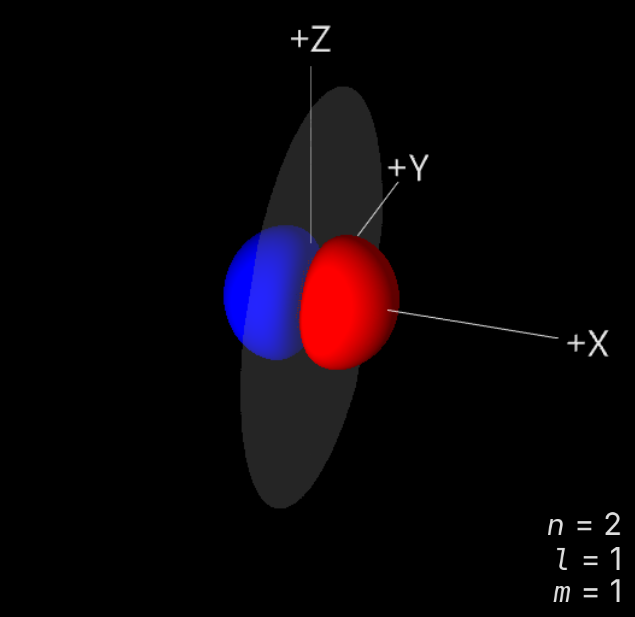
\includegraphics[width=0.35\textwidth]{Imagenes_QM/Orbital_comunmente.png}
\hspace{1cm}
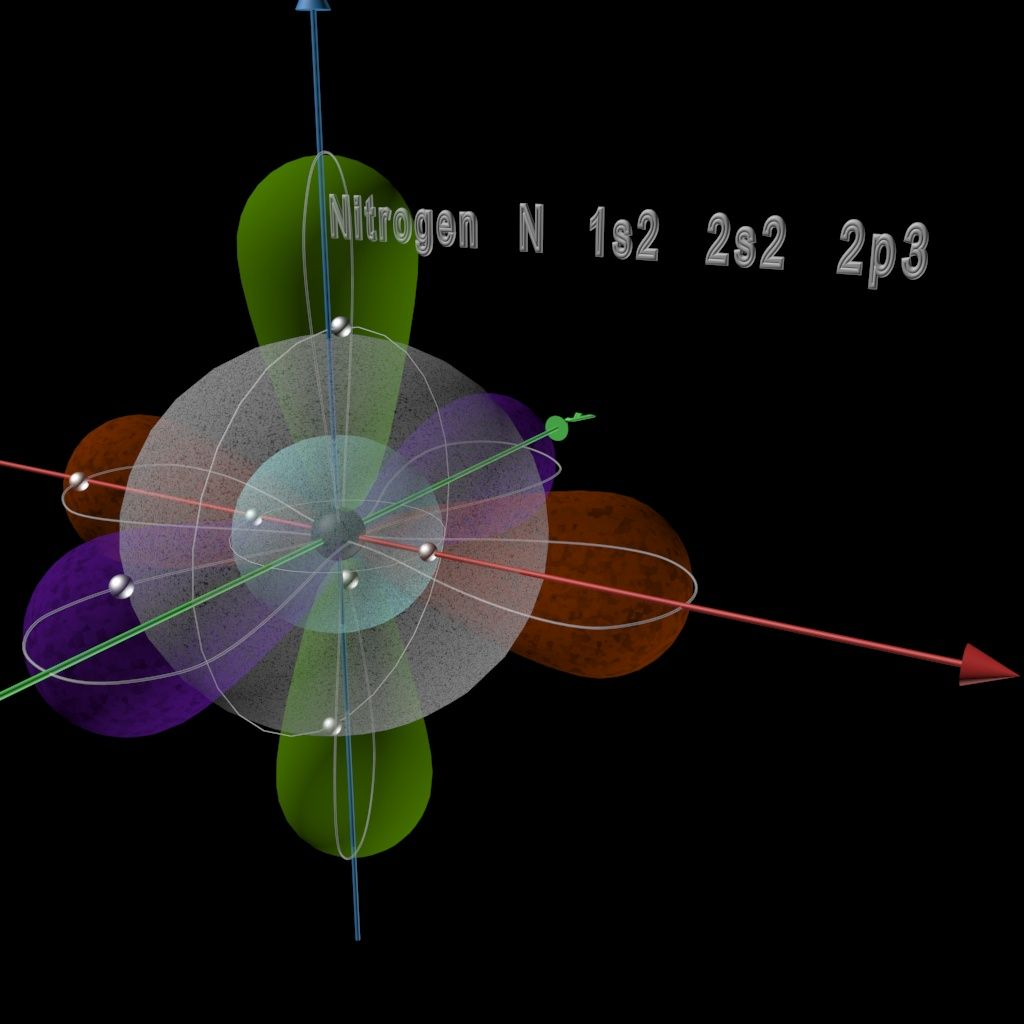
\includegraphics[width=0.45\textwidth]{Imagenes_QM/Orbitales_superpuestos.png}
\caption*{\small Izquierda: representación didáctica estándar de un orbital $2p$ aislado. 
Derecha: el nitrógeno real con todos sus orbitales superpuestos simultáneamente 
($1s^2\,2s^2\,2p^3$). En química se muestra el de la izquierda porque es el 
frontera relevante para la reactividad, no porque sea el único presente.}
\end{figure}

\phantomsection
\label{sec:anexo:tom:cloa}
\textbf{A.1.3 Cómo se forman los orbitales moleculares: CLOA}

Cuando dos átomos se acercan, sus funciones de onda se solapan. La Combinación Lineal de Orbitales
Atómicos (CLOA) establece que $n$ orbitales atómicos producen exactamente $n$ orbitales
moleculares: no se crean ni destruyen, se transforman. Dos orbitales atómicos producen
obligatoriamente un orbital enlazante y uno antienlazante. \\

\phantomsection
\label{sec:anexo:tom:enlazante}
\textbf{A.1.4 Por qué el enlazante es de menor energía}

Las funciones de onda tienen fase (signo matemático). Cuando dos orbitales atómicos se combinan
\textit{en fase} (interferencia constructiva), las funciones de onda se refuerzan en la región
entre los núcleos, aumentando la densidad electrónica ahí.

Un electrón en esa región está simultáneamente cerca de dos núcleos positivos: la atracción
electrostática es la suma de la atracción de ambos, lo cual es muy favorable. Además, esa densidad
actúa como pantalla que reduce la repulsión núcleo-núcleo. El mayor volumen que ocupa el electrón
también baja su energía cinética por el principio de Heisenberg. El sistema baja energía. \\

\phantomsection
\label{sec:anexo:tom:antienlazante}
\textbf{A.1.5 Por qué el antienlazante es de mayor energía}

Cuando dos orbitales se combinan \textit{en desfase} (interferencia destructiva), las funciones de
onda se cancelan entre los núcleos creando un \textbf{nodo}: densidad electrónica cero entre los
núcleos. El electrón está en los lóbulos \textit{externos}, lejos de ambos núcleos en promedio.
Sin pantalla electrónica, los núcleos se repelen sin amortiguación. El sistema sube de energía.

\textbf{Nota importante:} el orbital enlazante y el antienlazante \textit{no} ocupan regiones
separadas del espacio. Ambos se extienden por toda la región alrededor de los núcleos. Lo que
los diferencia es el patrón de densidad: el enlazante tiene su máximo entre los núcleos; el
antienlazante tiene densidad cero en el centro (nodo) y máximos en los extremos.

\begin{center}
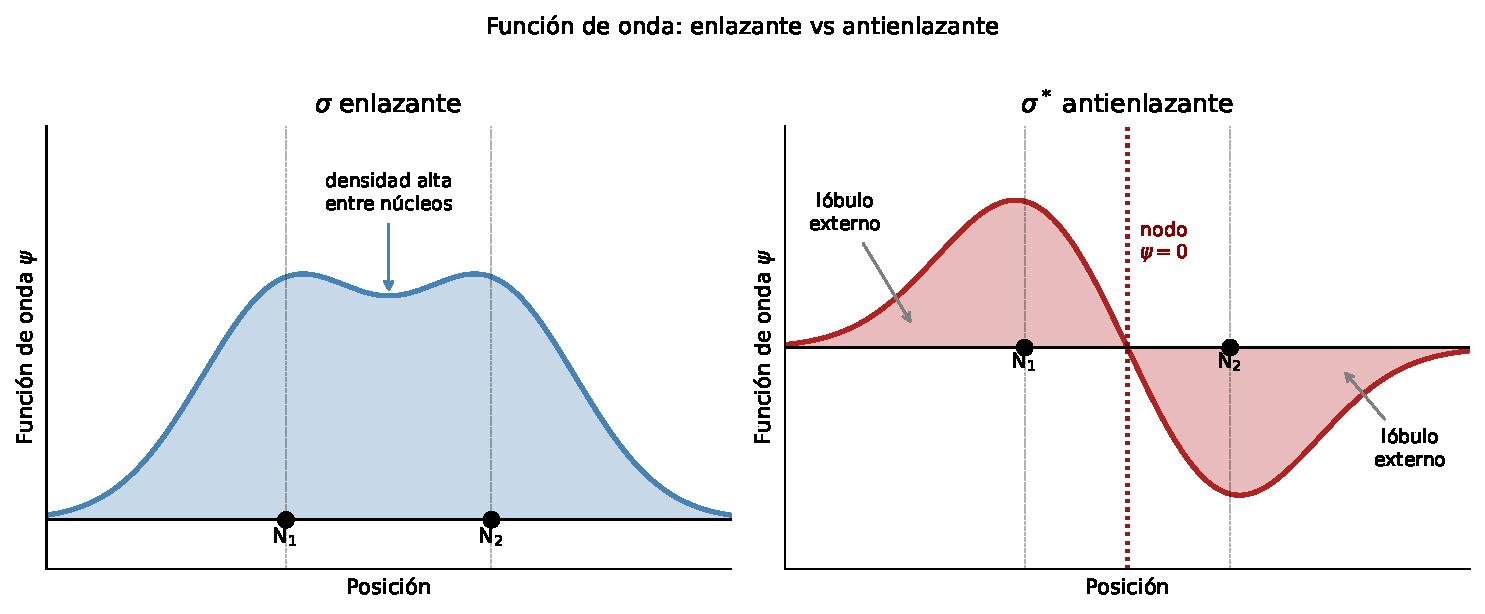
\includegraphics[width=0.85\textwidth]{Imagenes_QM/orbitales_enlace.pdf}
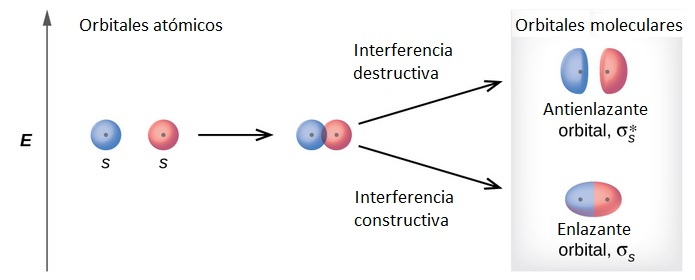
\includegraphics[width=0.85\textwidth]{Imagenes_QM/orbitales.png}
\end{center}

\phantomsection
\label{sec:anexo:tom:pauli}
\textbf{A.1.6 Por qué los electrones no se acumulan en el enlazante}

El enlazante es de menor energía, pero Pauli impide que más de dos electrones lo ocupen. El tercero
debe ir al $\sigma^*$. Esto no es intuitivo clásicamente, pero es consecuencia directa de que los
electrones ocupan estados cuánticos discretos, no espacio continuo. \\

\phantomsection
\label{sec:anexo:tom:orden}
\textbf{A.1.7 Orden de enlace}

\[
\text{O.E.} = \frac{e^- \text{ enlazantes} - e^- \text{ antienlazantes}}{2}
\]

O.E.$=0$: atracciones y repulsiones se cancelan exactamente, la molécula no existe.
Ejemplo: He$_2$ (2 enlazantes $-$ 2 antienlazantes $= 0$). \\

\phantomsection
\label{sec:anexo:tom:heisenberg}
\textbf{A.1.8 Por qué la deslocalización estabiliza: principio de incertidumbre de Heisenberg}

\[
\Delta x \cdot \Delta p \geq \frac{\hbar}{2}
\]

Si el electrón está más confinado en el espacio (menor $\Delta x$), su momento debe ser más
incierto (mayor $\Delta p$), lo que implica mayor energía cinética promedio. Si el electrón puede
ocupar mayor volumen (mayor $\Delta x$), su energía cinética promedio disminuye.

\textbf{Deslocalización:} extiende la nube del electrón hacia mayor volumen $\rightarrow$ menor
energía cinética por Heisenberg $\rightarrow$ sistema más estable.

\textbf{Polarización} (efecto inductivo): contrae la nube hacia un átomo electronegativo sin cambio
de orbital $\rightarrow$ menor volumen efectivo $\rightarrow$ mayor energía cinética $\rightarrow$
desestabiliza en radicales. \\

Mecanismo unificador de los efectos electrónicos según la especie:

\begin{center}
\small
\begin{tabular}{p{3.5cm}p{3cm}p{2cm}p{2cm}}
\hline
\textbf{Efecto} & \textbf{Mecanismo} & \textbf{Rad./Cat.} & \textbf{Carbanión} \\
\hline
Hiperconj. positiva & $\Delta x\uparrow$, $E_k\downarrow$ & Estabiliza & Desestabiliza \\
Hiperconj. negativa & $\Delta x\uparrow$, $E_k\downarrow$ & Estabiliza & Desestabiliza \\
Donación resonancia & $\Delta x\uparrow$, $E_k\downarrow$ & Estabiliza & Desestabiliza \\
Efecto inductivo & Heisenberg$\uparrow$ + Coulomb & Desestabiliza & Estabiliza \\
\hline
\end{tabular}
\normalsize
\end{center}

\textbf{Nota sobre el inductivo en carbaniones:} el efecto inductivo opera simultáneamente por
dos mecanismos opuestos. Por Heisenberg, contrae la nube electrónica aumentando la energía cinética,
lo que desestabiliza. Por Coulomb, retira el exceso de carga negativa del carbono central,
reduciendo la repulsión electrón-electrón, lo que estabiliza. En carbaniones el efecto Coulomb
supera al efecto Heisenberg y el resultado neto es estabilización. En radicales no hay exceso de
carga que aliviar, y Heisenberg domina sin competencia: el inductivo desestabiliza. \\

\phantomsection
\label{sec:anexo:tom:somo}
\textbf{A.1.9 El SOMO semilleno como estado de equilibrio}

El \textsc{somo} con un electrón es un estado intermedio estable. Añadirle un electrón lo acercaría
a un carbanión (exceso de carga negativa, menos estable). Quitarle el único electrón lo convertiría
en un carbocatión (déficit de carga, menos estable). Cualquier desviación del estado semilleno
desestabiliza. Por eso en radicales la deslocalización estabiliza no porque ``done carga'' al
\textsc{somo}, sino porque extiende el volumen del electrón que ya está ahí, bajando su energía
cinética sin alterar la ocupación del estado. \\

\phantomsection
\label{sec:anexo:tom:conexion}
\textbf{A.1.10 Conexión con los efectos del texto principal}

\begin{itemize}
\item \textbf{Hiperconjugación positiva:} los hidrógenos $\beta$ (átomos H unidos al carbono
$\alpha$, es decir a dos enlaces del carbono radical) solapan con el \textsc{somo}. El electrón
desapareado se extiende hacia esos enlaces. Mayor volumen, menor energía cinética, estabiliza.
\item \textbf{Hiperconjugación negativa:} el electrón del \textsc{somo} se extiende hacia el
$\sigma^*$ vacío del enlace C--H vecino alineado. Mayor volumen, menor energía cinética,
estabiliza. Contribuye a geometría ligeramente piramidal.
\item \textbf{Efecto inductivo (F en posición $\alpha$):} el F atrae la nube del \textsc{somo}
hacia sí. El electrón no se transfiere, solo se contrae espacialmente. Menor volumen, mayor
energía cinética, desestabiliza.
\item \textbf{Donación por resonancia (F en posición $\beta$):} el par libre del F solapa con
el \textsc{somo}. El electrón se extiende hacia ese par libre. Mayor volumen, estabiliza. Este
efecto compite con el inductivo del mismo F.
\end{itemize}

\phantomsection
\label{sec:anexo:tom:solapamiento}
\textbf{A.1.11 Por qué el solapamiento extiende la nube}

Cada orbital atómico es una función de onda $\psi$ localizada alrededor de su núcleo. Cuando dos
orbitales se acercan geométricamente y sus fases coinciden, las funciones de onda se suman
constructivamente. El orbital molecular resultante tiene mayor amplitud en esa región extendida,
y como la densidad es $|\psi|^2$, el electrón tiene mayor probabilidad de estar en ese volumen
más amplio.

Este solapamiento no forma un enlace nuevo. Es simplemente que las funciones de onda matemáticas
se superponen en el espacio por estar geométricamente alineadas y en fase. El electrón no se
transfiere, solo tiene mayor probabilidad de existir en mayor volumen. Por eso se llama
deslocalización parcial: la interacción es más débil que un enlace $\pi$ real (que requiere dos
electrones). \\

\textbf{Nota final de A.1:} la hibridación ($sp^2$, $sp^3$) y la \textsc{tev} son modelos
matemáticos sin existencia física propia. \textsc{tom} describe los electrones como estados
cuánticos moleculares sin necesidad de hibridación como concepto separado. El carácter $s$ de
un orbital es un concepto nativo de \textsc{tom} más fundamental que la hibridación discreta.

\phantomsection
\label{sec:anexo:tom:frontera}
\textbf{A.1.12 Orbitales frontera y reactividad}

De todos los orbitales superpuestos de un átomo, la química se simplifica 
enormemente mirando solo el \textbf{orbital frontera}: el que participa 
en la reacción. Según el contexto:
\begin{itemize}
\item \textbf{HOMO} (Highest Occupied Molecular Orbital): orbital lleno 
de mayor energía. Es desde donde dona el nucleófilo.
\item \textbf{LUMO} (Lowest Unoccupied Molecular Orbital): orbital vacío 
de menor energía. Es donde acepta el electrófilo.
\item \textbf{SOMO} (Singly Occupied Molecular Orbital): orbital con un 
solo electrón. Es el orbital del radical.
\end{itemize}

Los demás orbitales están ahí pero no determinan la reactividad en ese 
momento. Por eso en el carbocatión $sp^2$ se muestra el $2p_z$ vacío: 
es el LUMO, donde ataca el nucleófilo. En el radical se muestra el SOMO 
porque ahí está el electrón desapareado.

% ─────────────────────────────────────────────────────────────

\phantomsection
\label{sec:anexo:quiralidad}
\addcontentsline{toc}{subsubsection}{A.2 Quiralidad, enantiómeros y mezclas racémicas}
\subsubsection*{\textcolor{blueunam}{A.2 Quiralidad, enantiómeros y mezclas racémicas}}

Este apartado surge del análisis de la $SN^1$, que genera mezclas racémicas. Para entender
por qué, es necesario comprender qué es la quiralidad y cómo se relaciona con los isómeros
y las mezclas racémicas. \\

\phantomsection
\label{sec:anexo:quiralidad:isomeros}
\textbf{A.2.1 Isómeros}

Los isómeros son moléculas con la misma fórmula molecular pero diferente disposición de átomos.
Existen varios tipos:

\begin{itemize}
\item \textbf{Isómeros constitucionales:} difieren en la conectividad de los átomos.
\item \textbf{Estereoisómeros:} misma conectividad pero diferente disposición espacial.
Incluyen enantiómeros, diastereómeros y conformacionales.
\item \textbf{Enantiómeros:} estereoisómeros que son imágenes especulares no superponibles.
Solo existen cuando la molécula es quiral.
\item \textbf{Diastereómeros:} estereoisómeros que no son imágenes especulares entre sí.
\end{itemize}

\phantomsection
\label{sec:anexo:quiralidad:quiral}
\textbf{A.2.2 Quiralidad}

Un objeto es quiral cuando no es superponible a su imagen especular. En química, una molécula es
quiral cuando tiene al menos un \textbf{carbono quiral}: un carbono unido a cuatro sustituyentes
\textit{diferentes}. La quiralidad es una propiedad de la molécula, no un tipo de isomería.

Una molécula quiral no tiene propiedades físicas o químicas diferentes a su enantiómero en un
entorno aquiral. La diferencia aparece solo cuando interactúa con algo también quiral:

\begin{itemize}
\item \textbf{Luz polarizada:} un enantiómero la rota hacia la derecha (+) y el otro hacia la
izquierda ($-$). Esta propiedad se llama actividad óptica.
\item \textbf{Receptores biológicos:} los receptores son quirales, por eso un enantiómero puede
ser activo farmacológicamente y el otro inactivo o tóxico.
\item \textbf{Reactivos quirales:} reaccionan a velocidades diferentes con cada enantiómero.
\end{itemize}

\phantomsection
\label{sec:anexo:quiralidad:rs}
\textbf{A.2.3 Nomenclatura R y S}

Los enantiómeros se nombran según la configuración absoluta del carbono quiral usando las reglas
de Cahn-Ingold-Prelog (\textsc{cip}):

\begin{enumerate}
\item Asignar prioridades a los cuatro sustituyentes según número atómico (mayor $Z$ = mayor
prioridad).
\item Orientar la molécula con el sustituyente de menor prioridad apuntando hacia atrás.
\item Trazar una flecha de mayor a menor prioridad (1→2→3):
\begin{itemize}
\item Sentido horario → configuración \textbf{R} (\textit{rectus})
\item Sentido antihorario → configuración \textbf{S} (\textit{sinister})
\end{itemize}
\end{enumerate}

\phantomsection
\label{sec:anexo:quiralidad:rac}
\textbf{A.2.4 Mezcla racémica}

Una mezcla racémica es una mezcla en proporción 1:1 de los dos enantiómeros de un compuesto quiral.
No es un tipo de isomería sino una mezcla física. Se denota como $(\pm)$ o \textit{rac-}. No tiene
actividad óptica porque las rotaciones de ambos enantiómeros se cancelan exactamente. \\

\phantomsection
\label{sec:anexo:quiralidad:sn}
\textbf{A.2.5 Por qué $SN^1$ genera mezclas racémicas y $SN^2$ no}

En $SN^1$, el carbocatión intermedio es $sp^2$ y plano. El nucleófilo puede atacar con igual
probabilidad por la cara superior o inferior del orbital $p$ vacío, produciendo ambos enantiómeros
R y S en proporción 1:1: mezcla racémica.

En $SN^2$, el nucleófilo ataca exclusivamente por el lado opuesto al grupo saliente (ataque anti),
produciendo inversión de configuración (\textbf{inversión de Walden}): si el sustrato es R, el
producto es S, y viceversa. Un solo enantiómero.

\begin{center}
\small
\begin{tabular}{lll}
\hline
\textbf{Mecanismo} & \textbf{Estereoquímica} & \textbf{Resultado} \\
\hline
$SN^1$ & Ataque por ambas caras del carbocatión plano & Mezcla racémica $(\pm)$ \\
$SN^2$ & Ataque anti, inversión de Walden & Un solo enantiómero \\
\hline
\end{tabular}
\normalsize
\end{center}

\phantomsection
\label{sec:anexo:nucleofilicidad}
\addcontentsline{toc}{subsubsection}{A.3 Nucleofilicidad y polarizabilidad}
\subsubsection*{\textcolor{blueunam}{A.3 Nucleofilicidad y polarizabilidad}}

\phantomsection
\label{sec:anexo:nucleofilicidad:polar}
\textbf{A.3.1 Polarizabilidad}

La polarizabilidad es qué tan fácil se distorsiona la nube electrónica de 
un átomo bajo la influencia de un campo eléctrico externo. En átomos grandes, 
los electrones de valencia están lejos del núcleo y el efecto apantallante 
de los electrones internos reduce la atracción nuclear sobre ellos, haciendo 
que la nube sea extensa y fácil de deformar. En átomos pequeños la nube es 
compacta y rígida, más difícil de distorsionar.

Factores que aumentan la polarizabilidad:
\begin{itemize}
\item \textbf{Tamaño:} más grande $\Rightarrow$ más polarizable. 
Los electrones externos están más lejos del núcleo y menos atraídos por él.
\item \textbf{Electronegatividad baja:} el átomo retiene menos sus electrones 
y los dona más fácilmente.
\item \textbf{Número de electrones:} más electrones $\Rightarrow$ más 
apantallamiento $\Rightarrow$ electrones externos menos atraídos.
\end{itemize}

\phantomsection
\label{sec:anexo:nucleofilicidad:carga}
\textbf{A.3.2 Nucleofilicidad: carga vs polarizabilidad}

La nucleofilicidad no depende solo de la carga negativa sino también de la 
polarizabilidad. Hay una competencia entre dos efectos:

\begin{itemize}
\item \textbf{A favor de la carga:} mayor densidad de carga negativa 
$\Rightarrow$ mayor atracción electrostática hacia el electrófilo.
\item \textbf{A favor de la polarizabilidad:} nube más distorsionable 
$\Rightarrow$ mejor solapamiento orbital con el $\sigma^*$ del sustrato 
en el estado de transición de $SN^2$.
\end{itemize}

En $SN^2$ domina el \textbf{solapamiento orbital} (factor cinético). 
Por eso \ce{I-} es mejor nucleófilo que \ce{F-} aunque \ce{F} tenga 
mayor carga negativa: el \ce{I-} es grande y polarizable, puede 
distorsionar su nube para solapar bien con el $\sigma^*$ del C--X 
sin repeler tanto a los electrones del enlace. El \ce{F-} es pequeño 
y rígido, su densidad concentrada repele fuertemente antes de llegar 
al $\sigma^*$.

\phantomsection
\label{sec:anexo:nucleofilicidad:cn}
\textbf{A.3.3 El caso del \ce{CN-}: nucleófilo ambidente}

El \ce{CN-} puede atacar por el C o por el N. La carga negativa está 
en el N, lo que sugeriría ataque por N. Sin embargo en $SN^2$ con 
disolvente aprótico ataca por el \textbf{C} porque:

\begin{itemize}
\item El C es más polarizable que el N (menos electronegativo, retiene 
menos sus electrones).
\item Mayor polarizabilidad $\Rightarrow$ mejor solapamiento con el 
$\sigma^*$ del C--X en el estado de transición.
\item La polarizabilidad supera a la ventaja electrostática del N.
\end{itemize}

El producto es un nitrilo R--CN. En condiciones donde domina la 
electrostática (iónicas, termodinámicas) puede atacar por N dando 
isocianuro R--NC.

\phantomsection
\label{sec:anexo:nucleofilicidad:electro}
\textbf{A.3.4 Nucleófilo y electrófilo desde electrostática}

La atracción entre nucleófilo y electrófilo es \textbf{mutua}: ambos 
se atraen simultáneamente por electrostática. La convención de que 
``el nucleófilo ataca al electrófilo'' es solo una elección de 
perspectiva: se sigue el movimiento de los \textbf{electrones}, 
que van de donde sobran hacia donde faltan. Si se siguiera el 
movimiento del ``hueco'' electrónico la dirección sería opuesta, 
pero la física es la misma.

El sitio nucleofílico o electrofílico no tiene que ser toda la 
molécula. Es el átomo o enlace con mayor o menor densidad electrónica 
disponible. Ejemplos: en el etóxido \ce{CH3CH2O-} el nucleófilo es 
el \ce{O-}, no toda la molécula. En el benceno el nucleófilo es el 
sistema $\pi$, no los carbonos individualmente.

\phantomsection
\label{sec:anexo:nucleofilicidad:homo}
\textbf{A.3.5 $SN^2$ desde TOM: interacción HOMO-LUMO}

En $SN^2$ lo que realmente ocurre es una interacción 
\textbf{HOMO-LUMO}: el par libre del nucleófilo (HOMO) solapa con 
el $\sigma^*$ del enlace C--X (LUMO) por el lado opuesto al grupo 
saliente. Al llenarse el $\sigma^*$, el enlace C--X se debilita y 
se rompe simultáneamente con la formación del nuevo enlace C--Nu.

El ataque debe ser \textbf{anti a 180°} porque el lóbulo de mayor 
densidad del $\sigma^*$ está en el lado opuesto al X. Sin esa 
alineación no hay solapamiento y la reacción no ocurre.

La interacción HOMO-LUMO siempre estabiliza el sistema: el orbital 
de menor energía baja más de lo que sube el de mayor energía. Por 
eso la reacción es favorable a pesar de que el $\sigma^*$ tiene más 
energía que el $\sigma$.

%---------- Final del documento ----------%
\end{document}